\documentclass[12pt]{article}
\usepackage{amsmath}
\usepackage{graphicx}
\usepackage{adjustbox}
\usepackage{booktabs}
\usepackage{tabularx}
\usepackage{fullpage}
\usepackage{subcaption}
\usepackage{cite}
\usepackage{amsfonts}
\usepackage{float} % Added to allow [H] float specifier



\title{Spatio-Temporal Machine Learning for Economic Forecasting: A Cross-Indicator and Cross-Country Analysis Using World Bank Data}
\author{Jiadong Zhang\thanks{Email: \texttt{dereksodo@gmail.com}}}
\date{May 2025}

\begin{document}

\maketitle

\begin{abstract}
This paper develops a spatio-temporal framework for forecasting key macroeconomic indicators using machine learning techniques. Leveraging World Bank panel data from 1960 to 2020, we investigate three core tasks: (1) cross-indicator prediction—forecasting one major indicator based on others; (2) national-level time series forecasting; and (3) cross-national forecasting for major economies. Through comparative analysis of models including XGBoost, Random Forest, and linear baselines, we find that most structural indicators are highly predictable, while GDP growth remains volatile and difficult to model. We introduce a novel feasibility rate metric to assess reliability across multiple performance dimensions. Our results highlight both the promise and the limitations of data-driven methods in economic forecasting and underscore the importance of model selection, data context, and indicator stability.
\end{abstract}

\newpage
\tableofcontents
\newpage


\section{Introduction}

Macroeconomic indicators provide a comprehensive lens for assessing the economic and social development of countries. This study leverages World Bank panel data from 1960 to 2020 to identify key national indicators and evaluate their predictability using machine learning. The focus is on cross-indicator prediction: can one major indicator be reliably predicted from the others?
\section{Literature Review}

Recent advancements in machine learning (ML) have significantly influenced macroeconomic forecasting. This section reviews key studies that have explored the integration of ML techniques into economic prediction models.

\subsection{Nonlinearity and Regularization in ML Forecasting}

Goulet Coulombe et al. (2019) investigate the efficacy of ML in macroeconomic forecasting, emphasizing the importance of capturing nonlinear relationships in economic data. Their study concludes that nonlinearity is a crucial factor in improving forecast accuracy. They also highlight that traditional factor models serve as effective regularization tools within ML frameworks, aiding in managing model complexity and preventing overfitting. The authors advocate for the use of K-fold cross-validation as a best practice for model evaluation and selection. Their findings suggest that ML models, when properly regularized and validated, can outperform traditional econometric models, especially during periods of economic uncertainty and financial stress \cite{GouletCoulombe2019}.

\subsection{Automating Forecasting with ML Techniques}

Hall (2018) explores the application of ML methods to macroeconomic forecasting, focusing on the automation of model selection and parameter tuning. The study demonstrates that ML algorithms can process vast and complex datasets, identifying patterns that traditional models might overlook. Hall's analysis reveals that ML models can outperform both simple time-series models and consensus forecasts from professional economists, particularly in predicting short-term economic indicators like the unemployment rate. The research underscores the potential of ML to enhance forecasting accuracy by reducing reliance on manual model specification and expert judgment \cite{Hall2018}.

\subsection{ML Applications in China's GDP Forecasting}

Yang et al. (2024) apply various ML models to forecast China's quarterly real GDP growth, assessing their performance against traditional econometric models and expert forecasts. Their study finds that ML models generally achieve lower forecast errors, particularly during stable economic periods. However, during economic inflection points, expert forecasts may exhibit greater accuracy due to a more nuanced understanding of the macroeconomic environment. Additionally, the authors employ interpretable ML techniques to identify key variables influencing GDP fluctuations, providing insights into the underlying drivers of economic change \cite{Yang2024}.

\subsection{Synthesis and Implications for Current Research}

The reviewed studies collectively highlight the transformative impact of ML on macroeconomic forecasting. They demonstrate that ML models, with their ability to capture complex nonlinear relationships and process large datasets, can enhance forecast accuracy beyond traditional methods. These findings inform the current research by underscoring the importance of incorporating ML techniques into economic prediction models, particularly for analyzing cross-indicator relationships, time series data, and cross-country economic dynamics.
While the empirical studies reviewed above emphasize the technical advances of ML-based forecasting, it is equally important to align these findings with economic theory. For instance, the persistent unpredictability of GDP growth observed in both past studies and our own results echoes theoretical insights from the Solow growth model\cite{Solow1956}, which attributes long-term economic growth primarily to exogenous technological progress—a factor that is inherently difficult to observe or predict. Likewise, indicators such as life expectancy and energy consumption—which consistently achieve low RMSE/STD and MASE and high $R^2$ and DA—reflect long-term structural trends that are more stable and easier to model. The declining predictive value of agricultural output aligns with structural transformation theory, which explains the shift of economic activity from agriculture to industry and services as economies develop. By framing ML findings within established theoretical paradigms, this study highlights not only algorithmic performance but also its macroeconomic interpretability.\cite{Solow1956, Kuznets1971}

% This section should review key literature on macroeconomic forecasting using machine learning.
% Include comparisons of cross-indicator modeling, single-country time series forecasting, and international panel data approaches.
% Discuss how your work extends or differs from past studies such as Goulet Coulombe (2019), Hall (2018), and Yang et al. (2024).
\section{Data and Methods}

\subsection{Data Source}

\begin{itemize}
    \item World Bank Open Data, 1960--2020, including G20 expect African Union.
    \item Main dataset: [World Bank Data by Indicators](https://github.com/light-and-salt/World-Bank-Data-by-Indicators) (GitHub repository)
    \item We selected features with more than 60\% of relevant data present to minimize interpolation errors, resulting in a subset of 13 indicators. From these, we identified 10 relatively independent features for modeling, denoted $\{F_1, F_2, \ldots, F_{10}\}$.\footnote{Check Table \ref{tab:indicator_table} for details.}
\end{itemize}

\begin{table}[H]
    \centering
    \small
    \adjustbox{center}{
        \begin{tabular}{|c|c|}
            \hline
            \textbf{Indicator Code} & \textbf{Indicator Name} \\
            \hline
            SP.DYN.LE00.IN & Life expectancy at birth, total (years) \\
            SP.URB.TOTL.IN.ZS & Urban population (\% of total population) \\
            NV.AGR.TOTL.ZS & Agriculture, forestry, and fishing, value added (\% of GDP) \\
            EG.USE.PCAP.KG.OE & Energy use (kg of oil equivalent per capita) \\
            FS.AST.PRVT.GD.ZS & Assets of private sector banks to GDP (\%) \\
            NE.IMP.GNFS.ZS & Imports of goods and services (\% of GDP) \\
            NY.GDP.MKTP.CD & GDP (current US\$) \\
            NE.EXP.GNFS.ZS & Exports of goods and services (\% of GDP) \\
            NY.GDP.MKTP.KD.ZG & GDP growth (annual \%) \\
            EN.ATM.GHGT.KT.CE & Total greenhouse gas emissions (kt of CO$_2$  equivalent) \\
            \hline
        \end{tabular}
    }
    \caption{Indicator Table}
    \label{tab:indicator_table}
\end{table}

\subsection{Data Preprocessing}

\begin{itemize}
    \item Interpolated missing values for convenience.
    \item Constructed a country-year-feature panel: each row is a unique (country, year) pair.
\end{itemize}



\subsection{Machine Learning Models}

The following models are compared\footnote{See /src/DataProcessing/models.py for parameters}:
\begin{itemize}
    \item Linear Regression (LR)
    \item Ridge Regression
    \item Lasso Regression
    \item Elastic Net
    \item Support Vector Regression (SVR)
    \item Random Forest (RF)
    \item K-Nearest Neighbors (KNN)
    \item XGBoost
    \item Locally Weighted Regression (LWR)
\end{itemize}

\subsection{Experimental Setup}

\begin{itemize}
    \item \textbf{Year ranges:}
    \begin{itemize}
        \item Full period: 1960--2020
        \item Recent period: 2010--2020
    \end{itemize}
    \item \textbf{Cross-Validation:} 5-fold cross-validation is used for each prediction, averaging metrics across folds.
    \item \textbf{Evaluation Metrics:}
    \begin{itemize}
        \item Standardized error (RMSE/STD)~\cite{ChaiDraxler2014}, threshold = 1
        \item Coefficient of Determination ($R^2$)~\cite{Alexander2001}, threshold = 0.6
        \item Mean Absolute Scaled Error (MASE)~\cite{Hyndman2006}, threshold = 1
        \item Directional Accuracy (DA)~\cite{Hyndman2006}, threshold = 0.7
        \item \textbf{Guiding Metric (Heuristic Indicator):} For each model and indicator, we define a guiding metric score as the weighted score consisting of 4 metircs. Specifically, we compute:
        \begin{align*}
        \alpha_1 &= -\frac{\frac{\text{RMSE}_i}{\text{STD}_i} - 1}{1} \\\\
        \alpha_2 &= \frac{R_i^2 - 0.6}{0.6} \\\\
        \alpha_3 &= -\frac{\text{MASE}_i - 1}{1} \\\\
        \alpha_4 &= \frac{\text{DA}_i - 0.7}{0.7}
        \end{align*}
        \[
        \text{Guiding Score} = \sum_{i=1}^4 \frac{\beta_i}{1 + \exp(-\alpha_i)}
        \]
        $\beta_i$ is the weight assigned to each standard metric, and in this paper we choose $\beta = \{2.0, 2.0, 1.0, 5.0\}$ because when making policies the direction seems more important than the actual value. When all metrics are at their thresholds, Guiding Score = 2.0, also the threshold for Guiding Metric.
    \end{itemize}
    \item \textbf{Visualization:} For each model and year range, bar plots of the metrics are generated, with feasible region thresholds indicated.
\end{itemize}

\section{Cross-Indicator Forecasting}

\subsection{Prediction Task}
For each indicator $F_k$, we predict its value for each country-year using the remaining 9 indicators as input features. The process is repeated for all $k = 1, \ldots, 10$.
\subsection{Prediction Results}
% Retain your current performance evaluation here.

% Sample Figure Placeholders
\begin{figure}[h]
    \centering
    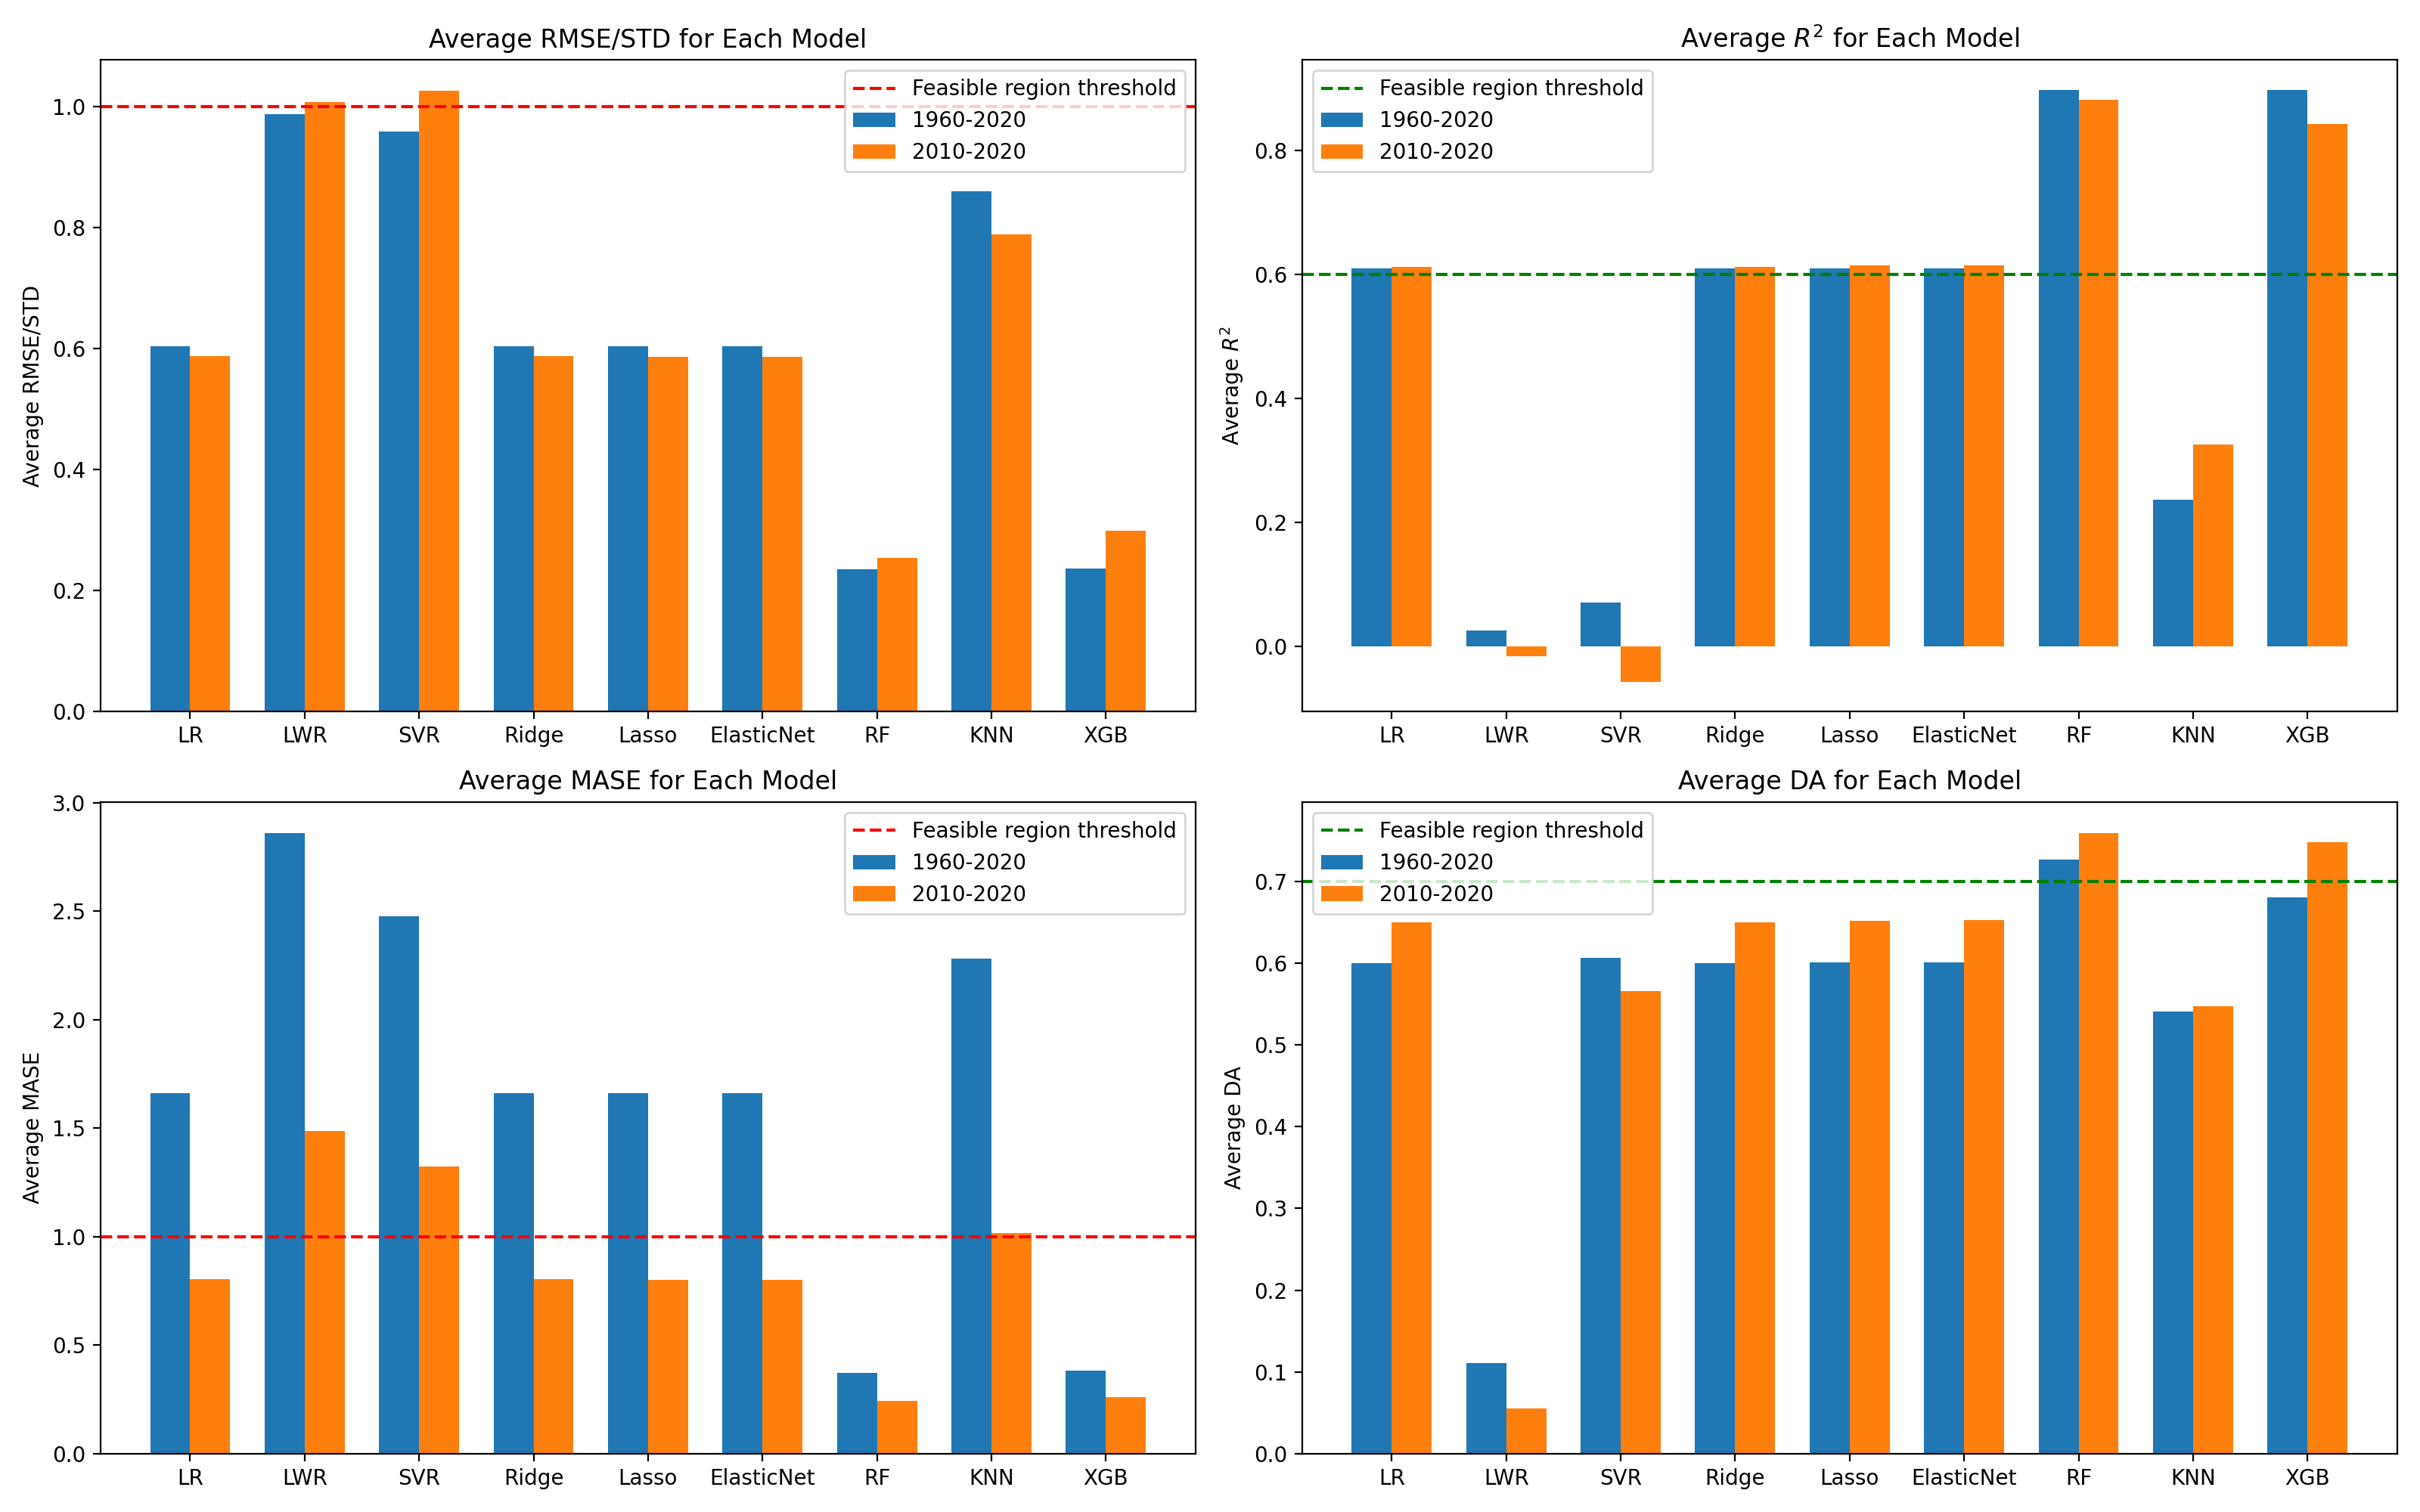
\includegraphics[width = \linewidth]{Combined_Metrics_figure1.png}
    
    \caption{Comparison of Model Performance: RMSE/STD, $R^2$, MASE and DA (1960–2020, 2010–2020)}
    \label{fig:model_compare_1}
\end{figure}
\begin{figure}[H]
    \centering
    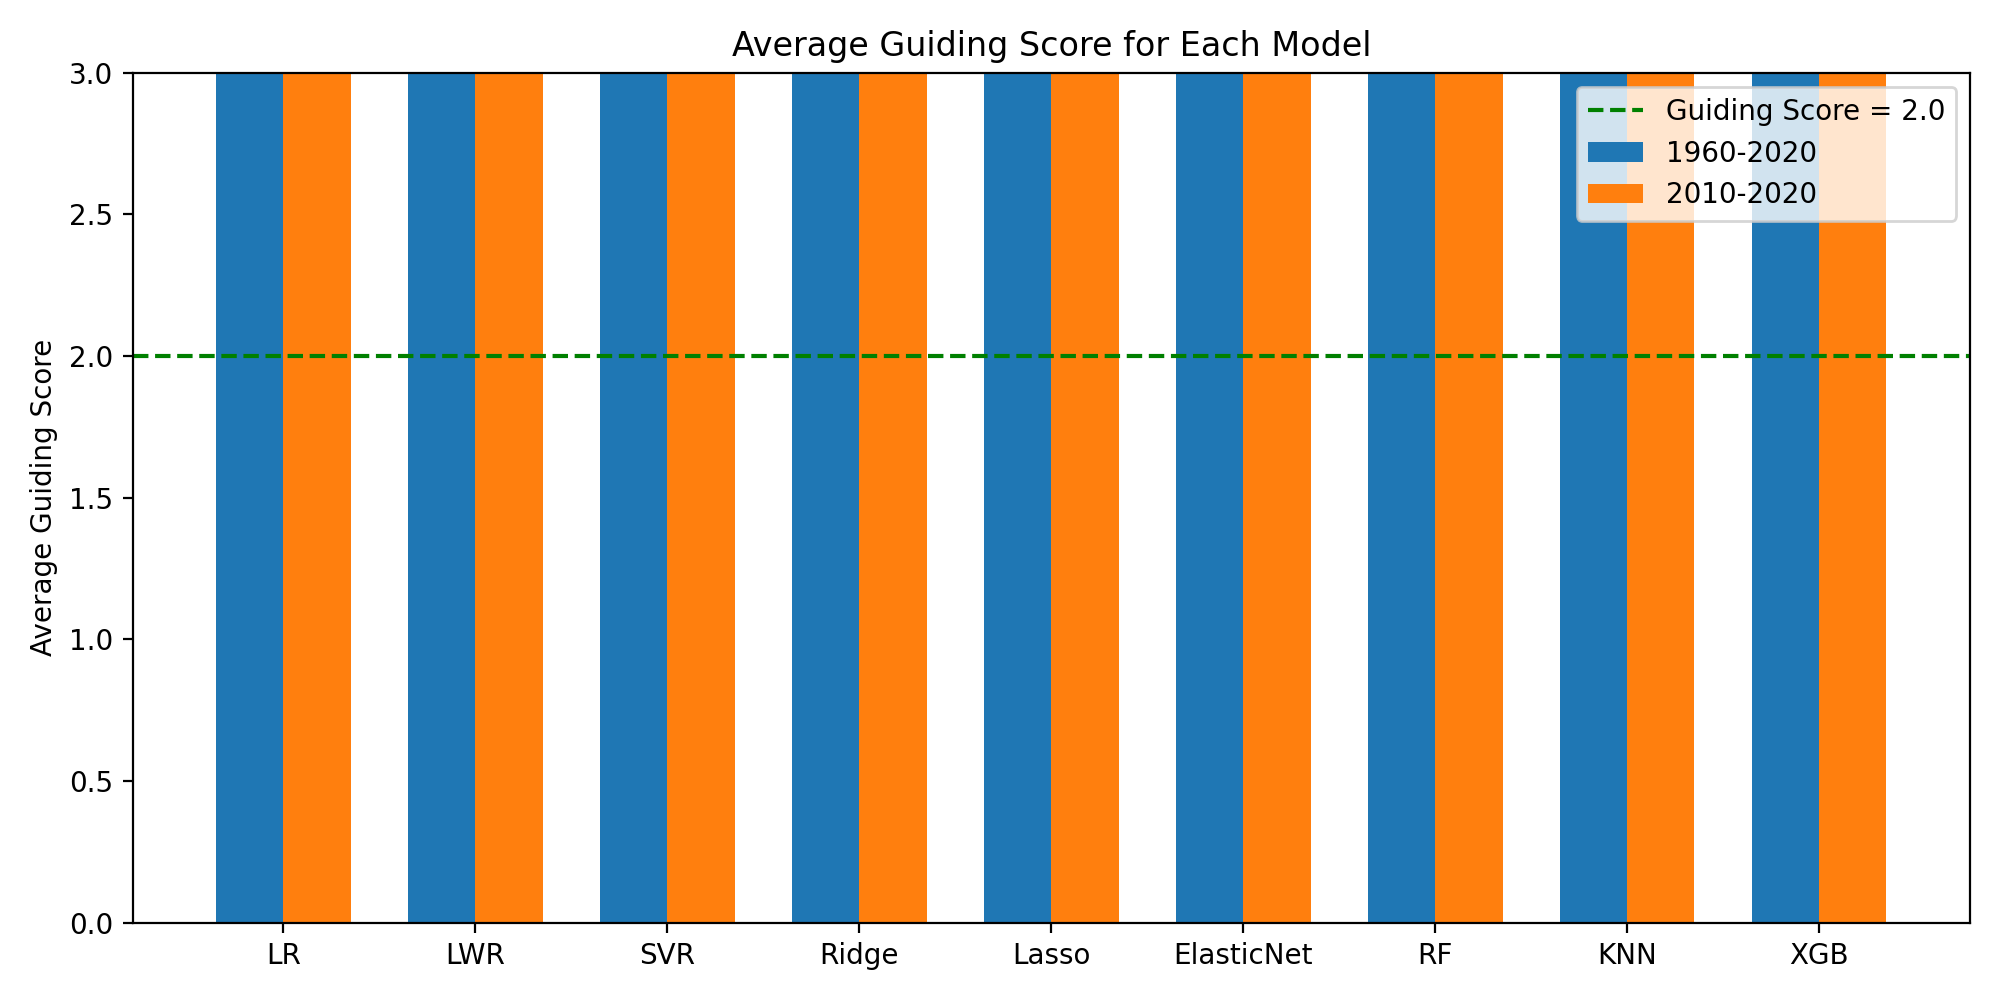
\includegraphics[width = \linewidth]{Average_GuidingScore_figure2.png}
    \caption{Comparison of Model Performance: Guiding Score (1960–2020, 2010–2020)}
    \label{fig:model_compare_2}
\end{figure}
\begin{figure}[H]
    \centering
    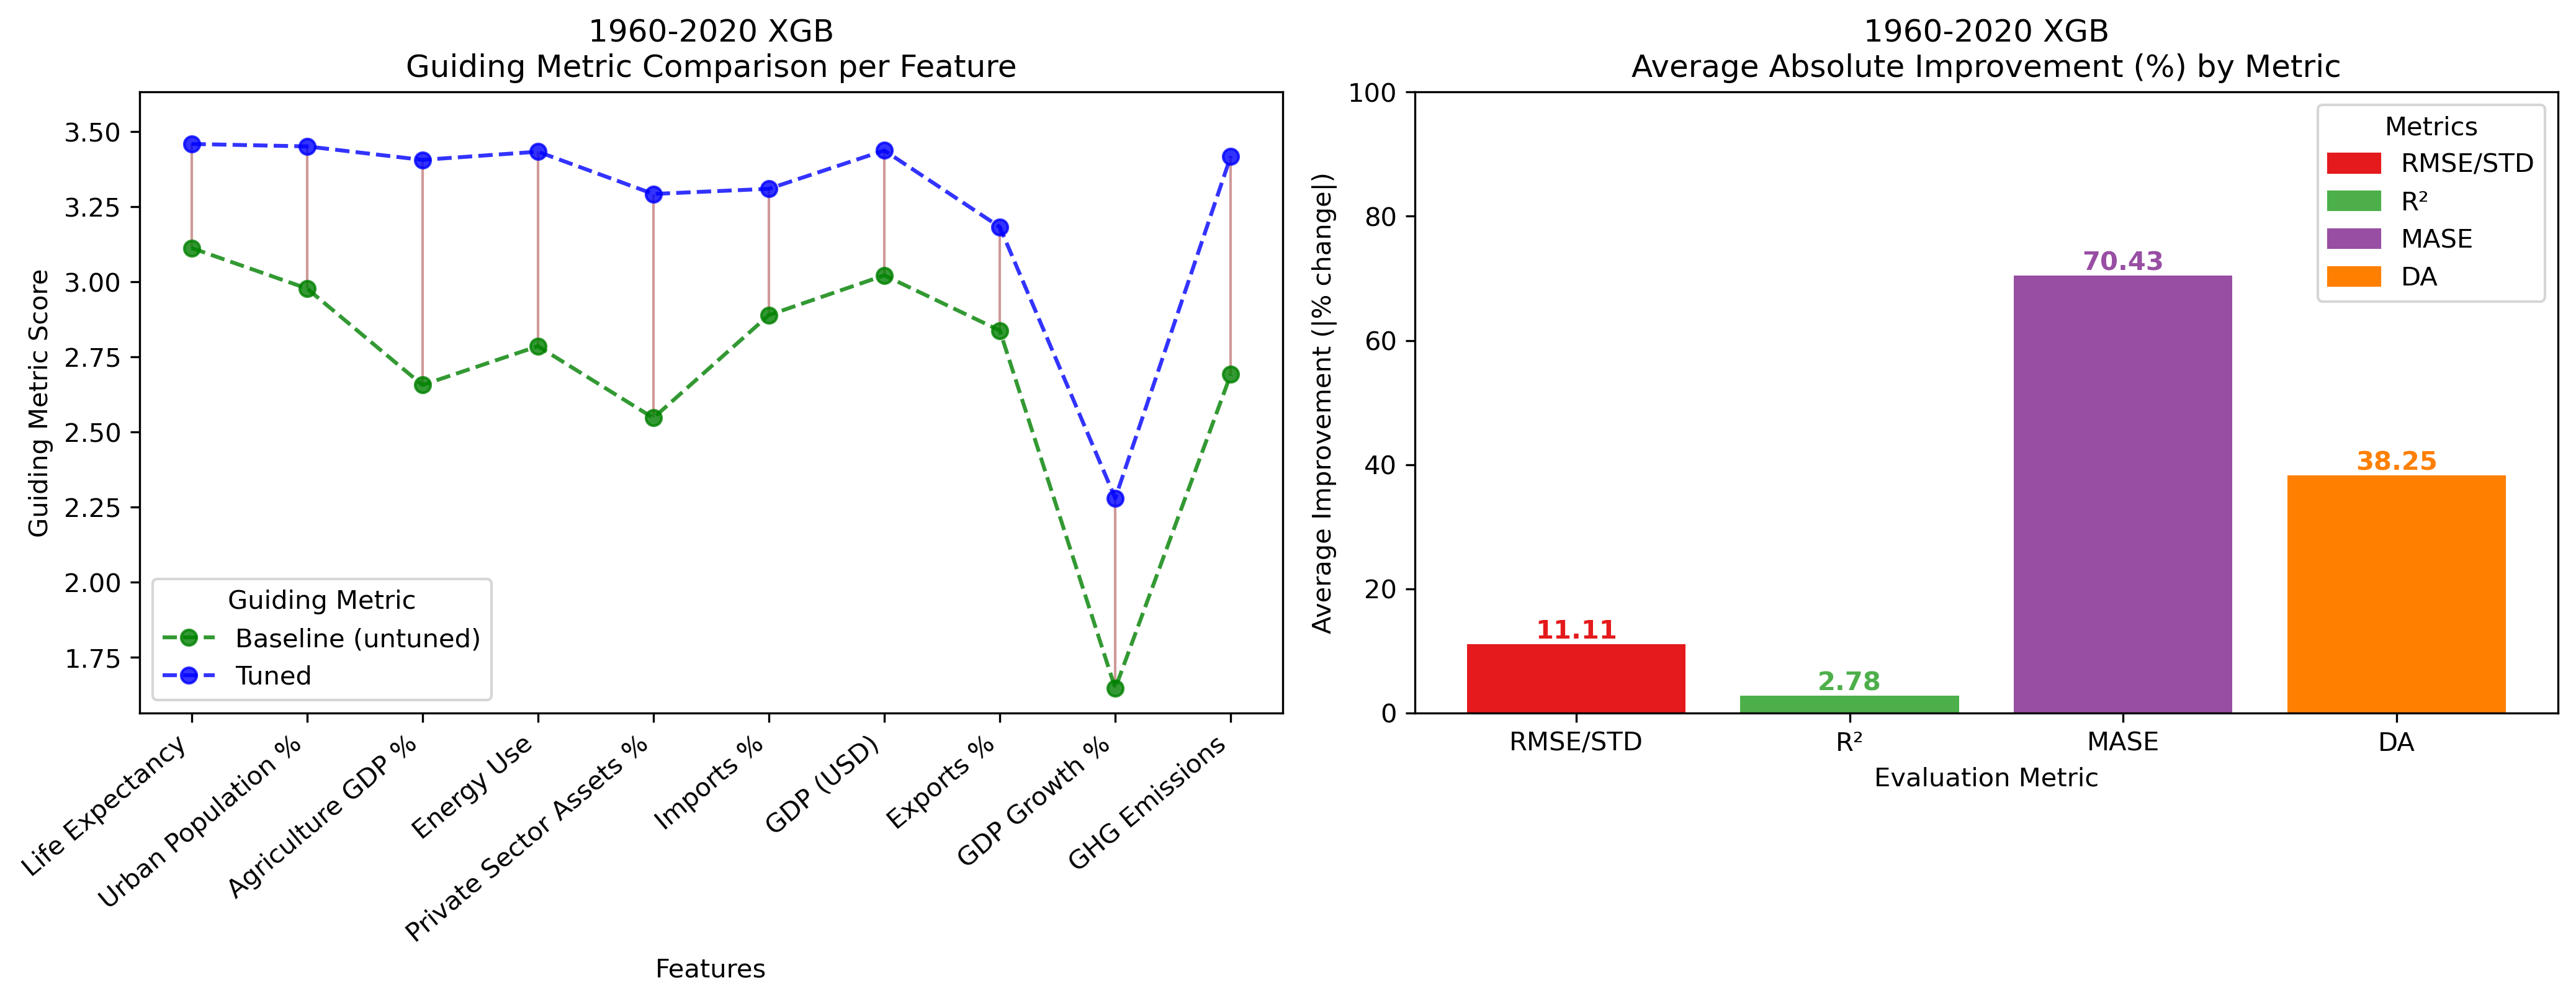
\includegraphics[width=\textwidth]{1960_2020_XGB_metrics.png}
    \caption{Prediction performance of XGBoost for each feature (1960--2020), including RMSE/STD, $R^2$, MASE, and Directional Accuracy.}
    \label{fig:xgb_feature_summary}
\end{figure}



From Figure~\ref{fig:model_compare_1} and Figure~\ref{fig:model_compare_2}, We can divide the chosen Machine Learning algorithms into 3 different categories: 
\begin{itemize}
\item RF and XGB have best performances, both of which has a low standardized error, MASE and high $R^2$ and DA, with a guiding score over 2.5
\item LR, Ridge, Lasso, ElasticNet have very similar performances, with a guiding score about 2.0 (2010-2020)
\item LWR, SVR, KNN have comparatively low performances. This is in part because the sample size (M = 1220 or 220) is rather small compared to input features (N = 10)
\end{itemize}
Figure~\ref{fig:xgb_feature_summary} summarizes the prediction performance of XGBoost for each of the 10 selected indicators over the full period (1960--2020). The results indicate that XGBoost achieves high accuracy for most structural indicators, with standardized errors (RMSE/STD) well below 1 and $R^2$ values typically above 0.6. Notably, indicators such as life expectancy, urban population share, and energy use are predicted with particularly high precision. In contrast, GDP growth (annual \%) stands out as the only indicator with consistently poor predictive performance, exhibiting both high error and low explanatory power. The poor predictability of the GDP growth rate compared to other major indicators is primarily due to its intrinsic volatility, exposure to a broad set of unobserved influences, and its weak contemporaneous linkages with slow-moving structural features. This is a well-documented phenomenon in economic modeling ~\cite{Loungani2001, ClementsHendry2002}, where forecasting economic growth remains an exceptionally challenging task.


\subsection{Hyperparameter Tuning}

To ensure robust performance from the ensemble models, we conducted hyperparameter tuning for both XGBoost (XGB) and Random Forest (RF) using grid search with 5-fold cross-validation.

For XGBoost, the primary hyperparameters adjusted include:
\begin{itemize}
    \item \texttt{n\_estimators}: Number of boosting rounds.
    \item \texttt{max\_depth}: Maximum depth of each tree.
    \item \texttt{learning\_rate}: Step size shrinkage used in updates.
    \item \texttt{subsample}: Fraction of observations to be randomly sampled for each tree.
    \item \texttt{colsample\_bytree}: Fraction of columns to be randomly sampled for each tree.
\end{itemize}

For Random Forest, the tuning focused on:
\begin{itemize}
    \item \texttt{n\_estimators}: Number of trees in the forest.
    \item \texttt{max\_depth}: Maximum depth of the tree.
    \item \texttt{min\_samples\_split}: Minimum number of samples required to split an internal node.
    \item \texttt{max\_features}: Number of features to consider when looking for the best split.
\end{itemize}
\begin{figure}[H]
    \centering
    \begin{subfigure}[t]{0.9\textwidth}
        \centering
        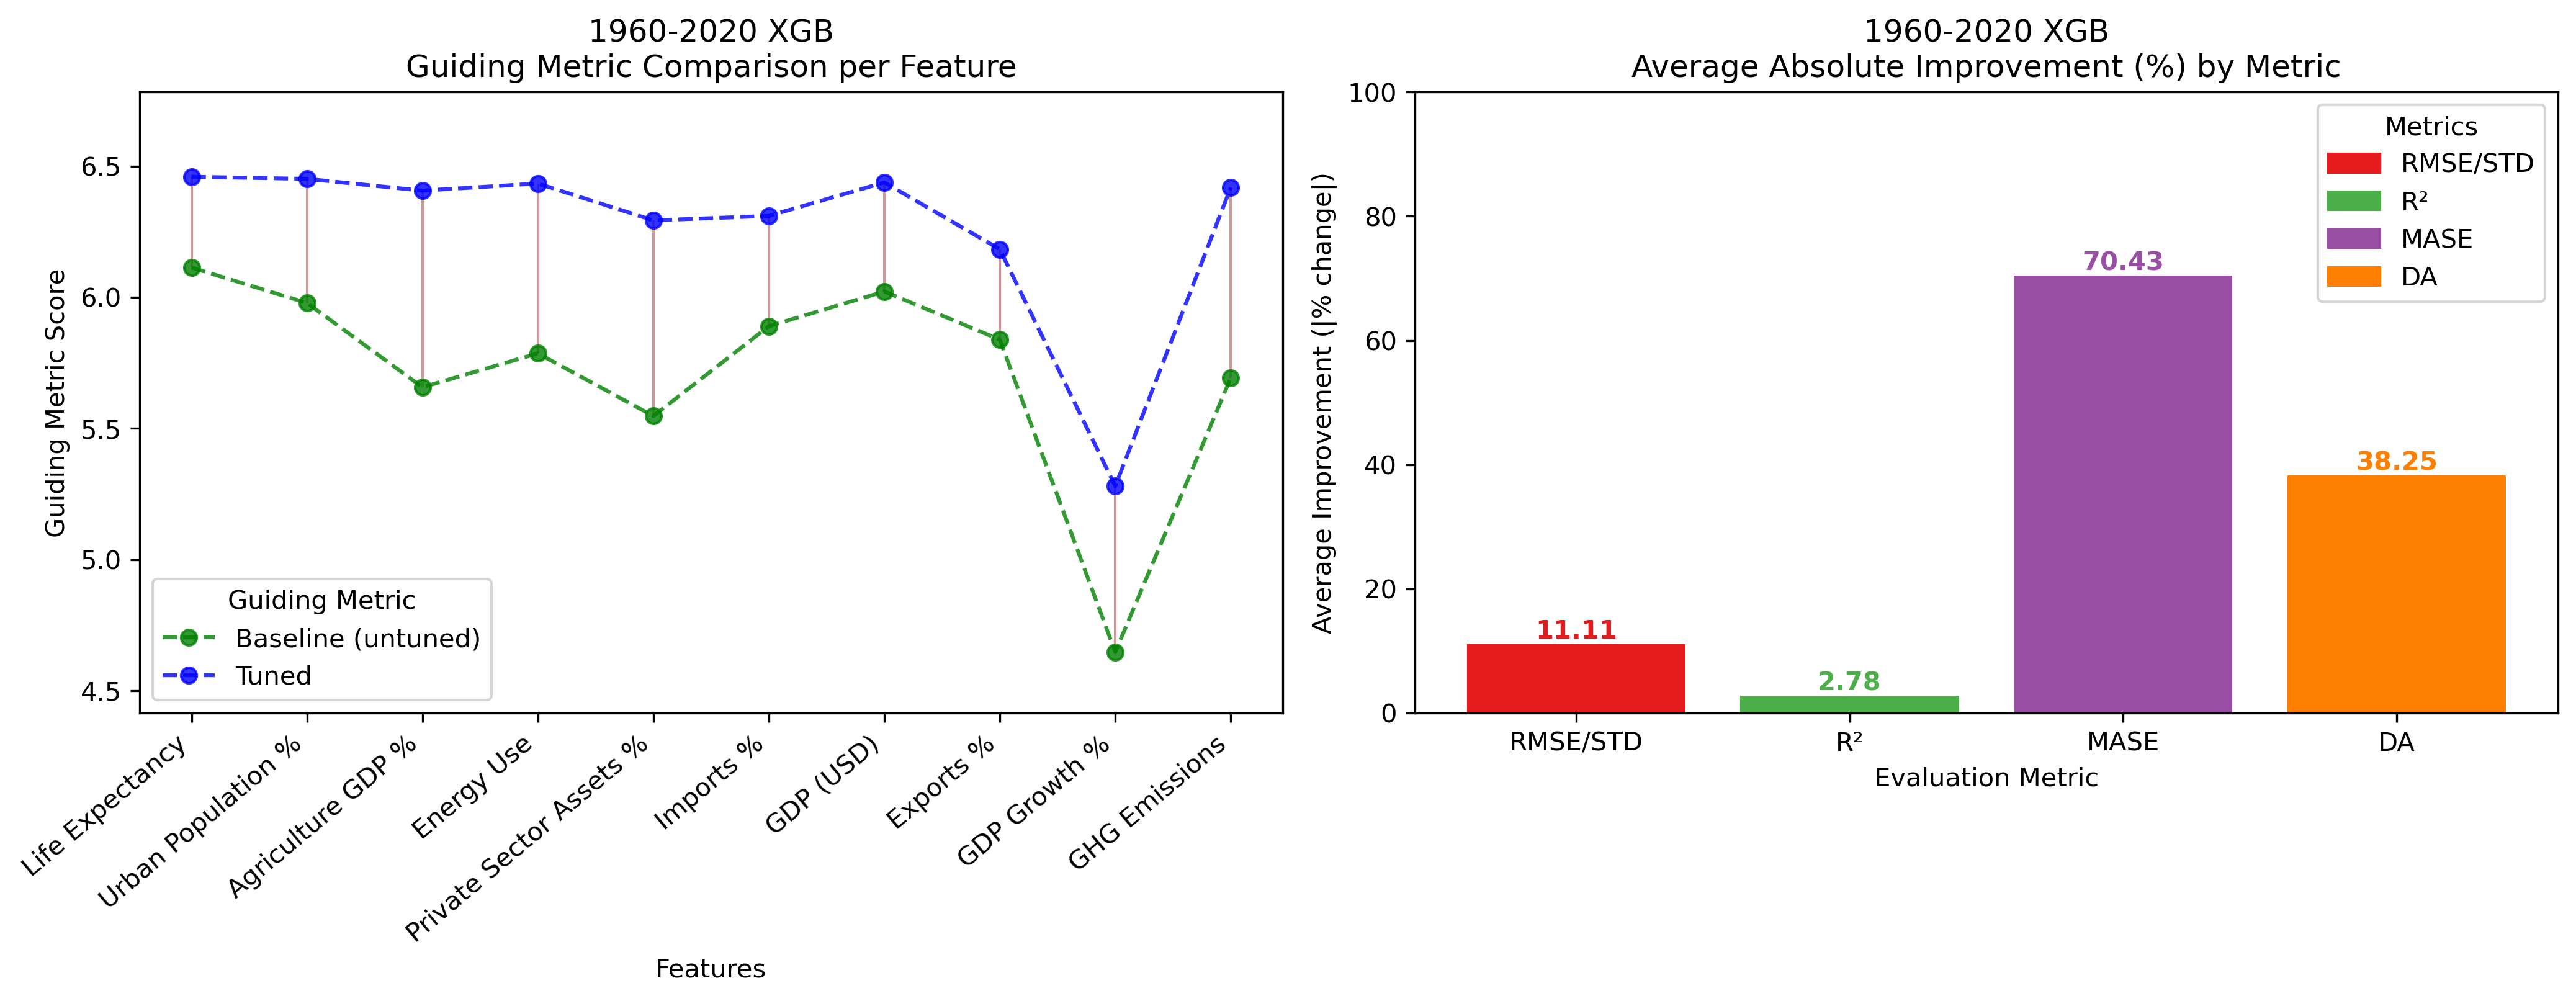
\includegraphics[width=\linewidth]{1960_2020_XGB_tuning_metrics.png}
        \caption{XGBoost: Tuning Performance (1960--2020)}
        \label{fig:xgb_tuning_1960_2020}
    \end{subfigure}
    \vspace{1em}
    \begin{subfigure}[t]{0.9\textwidth}
        \centering
        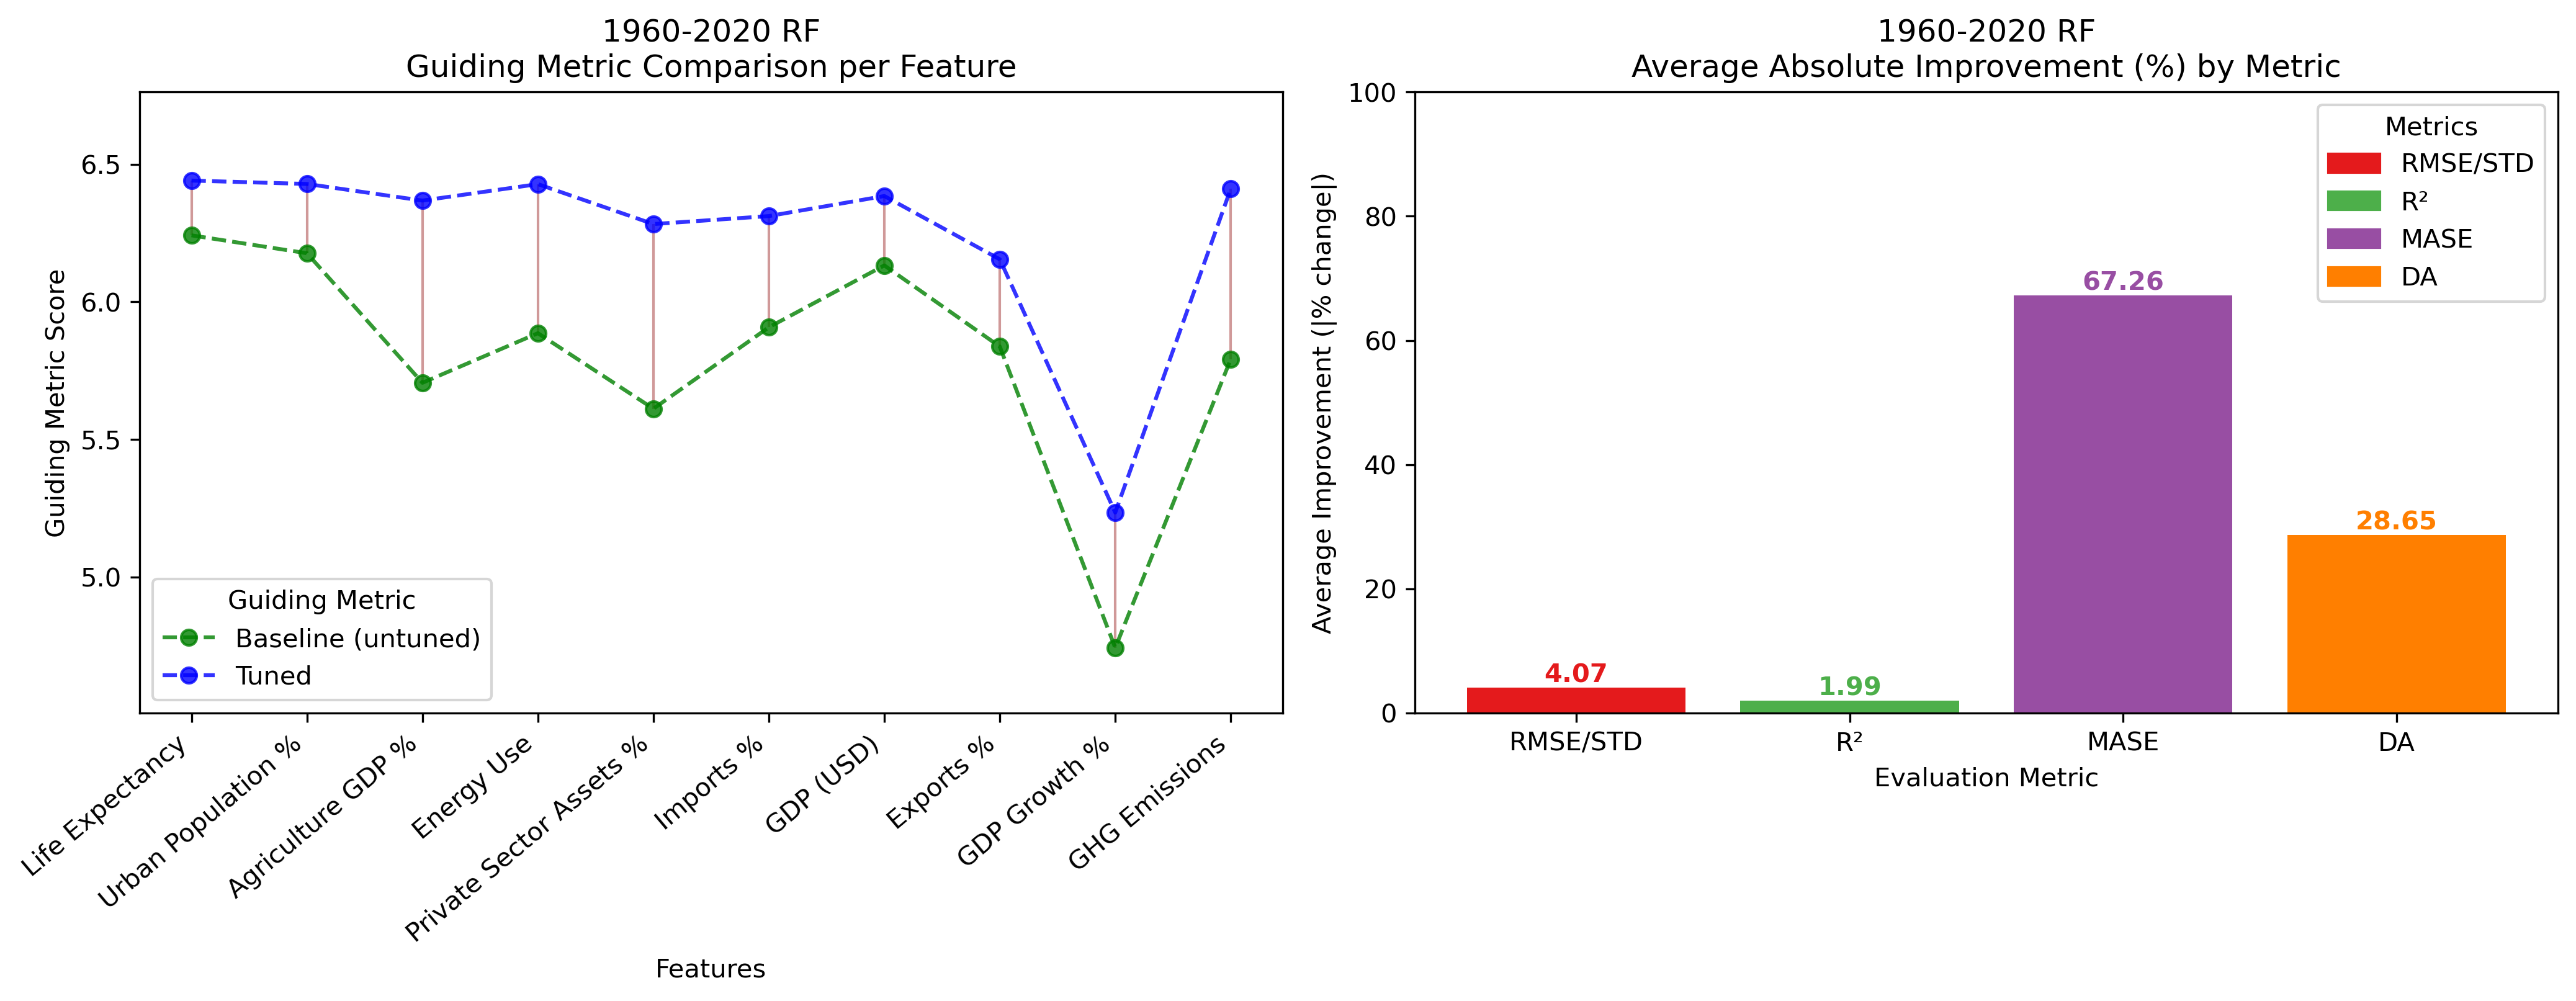
\includegraphics[width=\linewidth]{1960_2020_RF_tuning_metrics.png}
        \caption{Random Forest: Tuning Performance (1960--2020)}
        \label{fig:rf_tuning_1960_2020}
    \end{subfigure}
    \caption{Comparison of Hyperparameter Tuning Effects for XGBoost and Random Forest (1960--2020)}
    \label{fig:tuning_combined}
\end{figure}
Figure~\ref{fig:tuning_combined} illustrates how hyperparameter tuning improves model performance. Across all indicators, XGBoost consistently outperforms Random Forest, and both models benefit significantly from tuning.

Metric-wise, the most notable improvements appear in Directional Accuracy (DA), which rises by 30--40\%. This suggests that tuning not only improves numerical accuracy but also strengthens the models' ability to correctly predict the direction of change—a crucial feature for real-world policy and decision-making. Improvements in RMSE/STD and MASE are also evident, especially for structural indicators. In contrast, $R^2$ gains are modest, indicating that tuning has limited effect on variance explanation but substantial effect on practical usability.

Overall, tuning contributes most to directional consistency and error reduction, making ensemble models more robust and interpretable across diverse indicators.

Figure~\ref{fig:tuning_combined} provides a detailed visualization of the performance improvements after tuning. The left panel illustrates that while the magnitude of improvement of guiding score varies across indicators, all ten features experience a substantial average enhancement. This confirms that tuning has universal benefit, though its effect size depends on feature characteristics.

The right panel decomposes improvements across the four evaluation metrics. Notably, tuning yields minimal changes in $R^2$ (near 2\%), modest gains in RMSE/STD (ranging from 5\% to 10\%), and substantial improvements in Directional Accuracy (DA), which increase by approximately 30\%--40\%. The most dramatic effect is observed in Mean Absolute Scaled Error (MASE), where XGBoost and Random Forest achieves a nearly 70\% improvement. 
These results highlight how hyperparameter tuning differentially impacts specific model objectives and offer insights into which dimensions of forecast accuracy are most tunable.

\subsection{Summary}

Chapter 4 evaluated the feasibility of cross-indicator forecasting using machine learning models applied to national-level economic and social data. By predicting each indicator from the remaining features, we tested nine models across two time periods (1960–2020 and 2010–2020), and evaluated their performance using a composite guiding score.

XGBoost and Random Forest consistently outperformed other models, supporting the broader literature on the strengths of ensemble methods in capturing nonlinear macroeconomic patterns~\cite{Mullainathan2017ML, Athey2019ML}. Structural indicators—such as life expectancy, urban population, and energy use—were highly predictable, showing low error and strong directional accuracy. In contrast, GDP growth remained inherently difficult to forecast due to volatility and external shocks~\cite{Loungani2001, ClementsHendry2002}.

Model performance also improved in the 2010–2020 window, likely reflecting better data quality and macroeconomic convergence across countries~\cite{Baldwin2016Great, Jerven2013Poor}. These results emphasize the importance of model type, indicator stability, and temporal context in determining forecast reliability.

In summary, ensemble-based machine learning models, when properly tuned and evaluated with a balanced metric like the guiding score, offer a robust framework for forecasting slow-moving national indicators. This lays a solid foundation for the time-series and cross-national forecasting explored in subsequent chapters.


\section{Country-Level Time Series Forecasting}


\subsection{Dataset and Feature Construction}

This chapter uses the same interpolated dataset from 1960 to 2020 as in Chapter 4, including all available countries. For each of the 10 selected key indicators, we constructed lag-based time series features to facilitate temporal prediction modeling. Specifically, we created lag-2 and lag-3 versions of all other features (excluding the target) to predict each target feature value year by year.

The resulting time series dataset preserves the year and country code metadata, and ensures that the predictive modeling process incorporates temporal dynamics. All features were standardized prior to modeling to avoid scale issues.

\subsection{Models and Design Logic}

We evaluated six models for each country and each target indicator:

\begin{itemize}
    \item \textbf{Naive Forecast}: Uses the value of the previous year as the prediction for the next year.
    \item \textbf{ARIMA}: A univariate autoregressive model applied independently to each target series.
    \item \textbf{Rolling XGB-lag2}: Same as XGB-lag2, but predictions are generated year-by-year using only prior data up to that year (rolling forecast).
    \item \textbf{Rolling XGB-lag3}: Extends the rolling forecast logic to lag-3 input features.
\end{itemize}

The rolling forecast strategy better simulates real-world forecasting where future data is unavailable during training. The comparison across static and rolling variants allows us to evaluate model generalizability and robustness over time.

\subsection{Model Comparison}

% Compare forecasting performance of different time series models on a selected country.
% ------------------------------ Figure 6 Analysis ------------------------------
\subsubsection*{Country-Level Model Performances Analysis}
\begin{figure}[H]
    \centering
    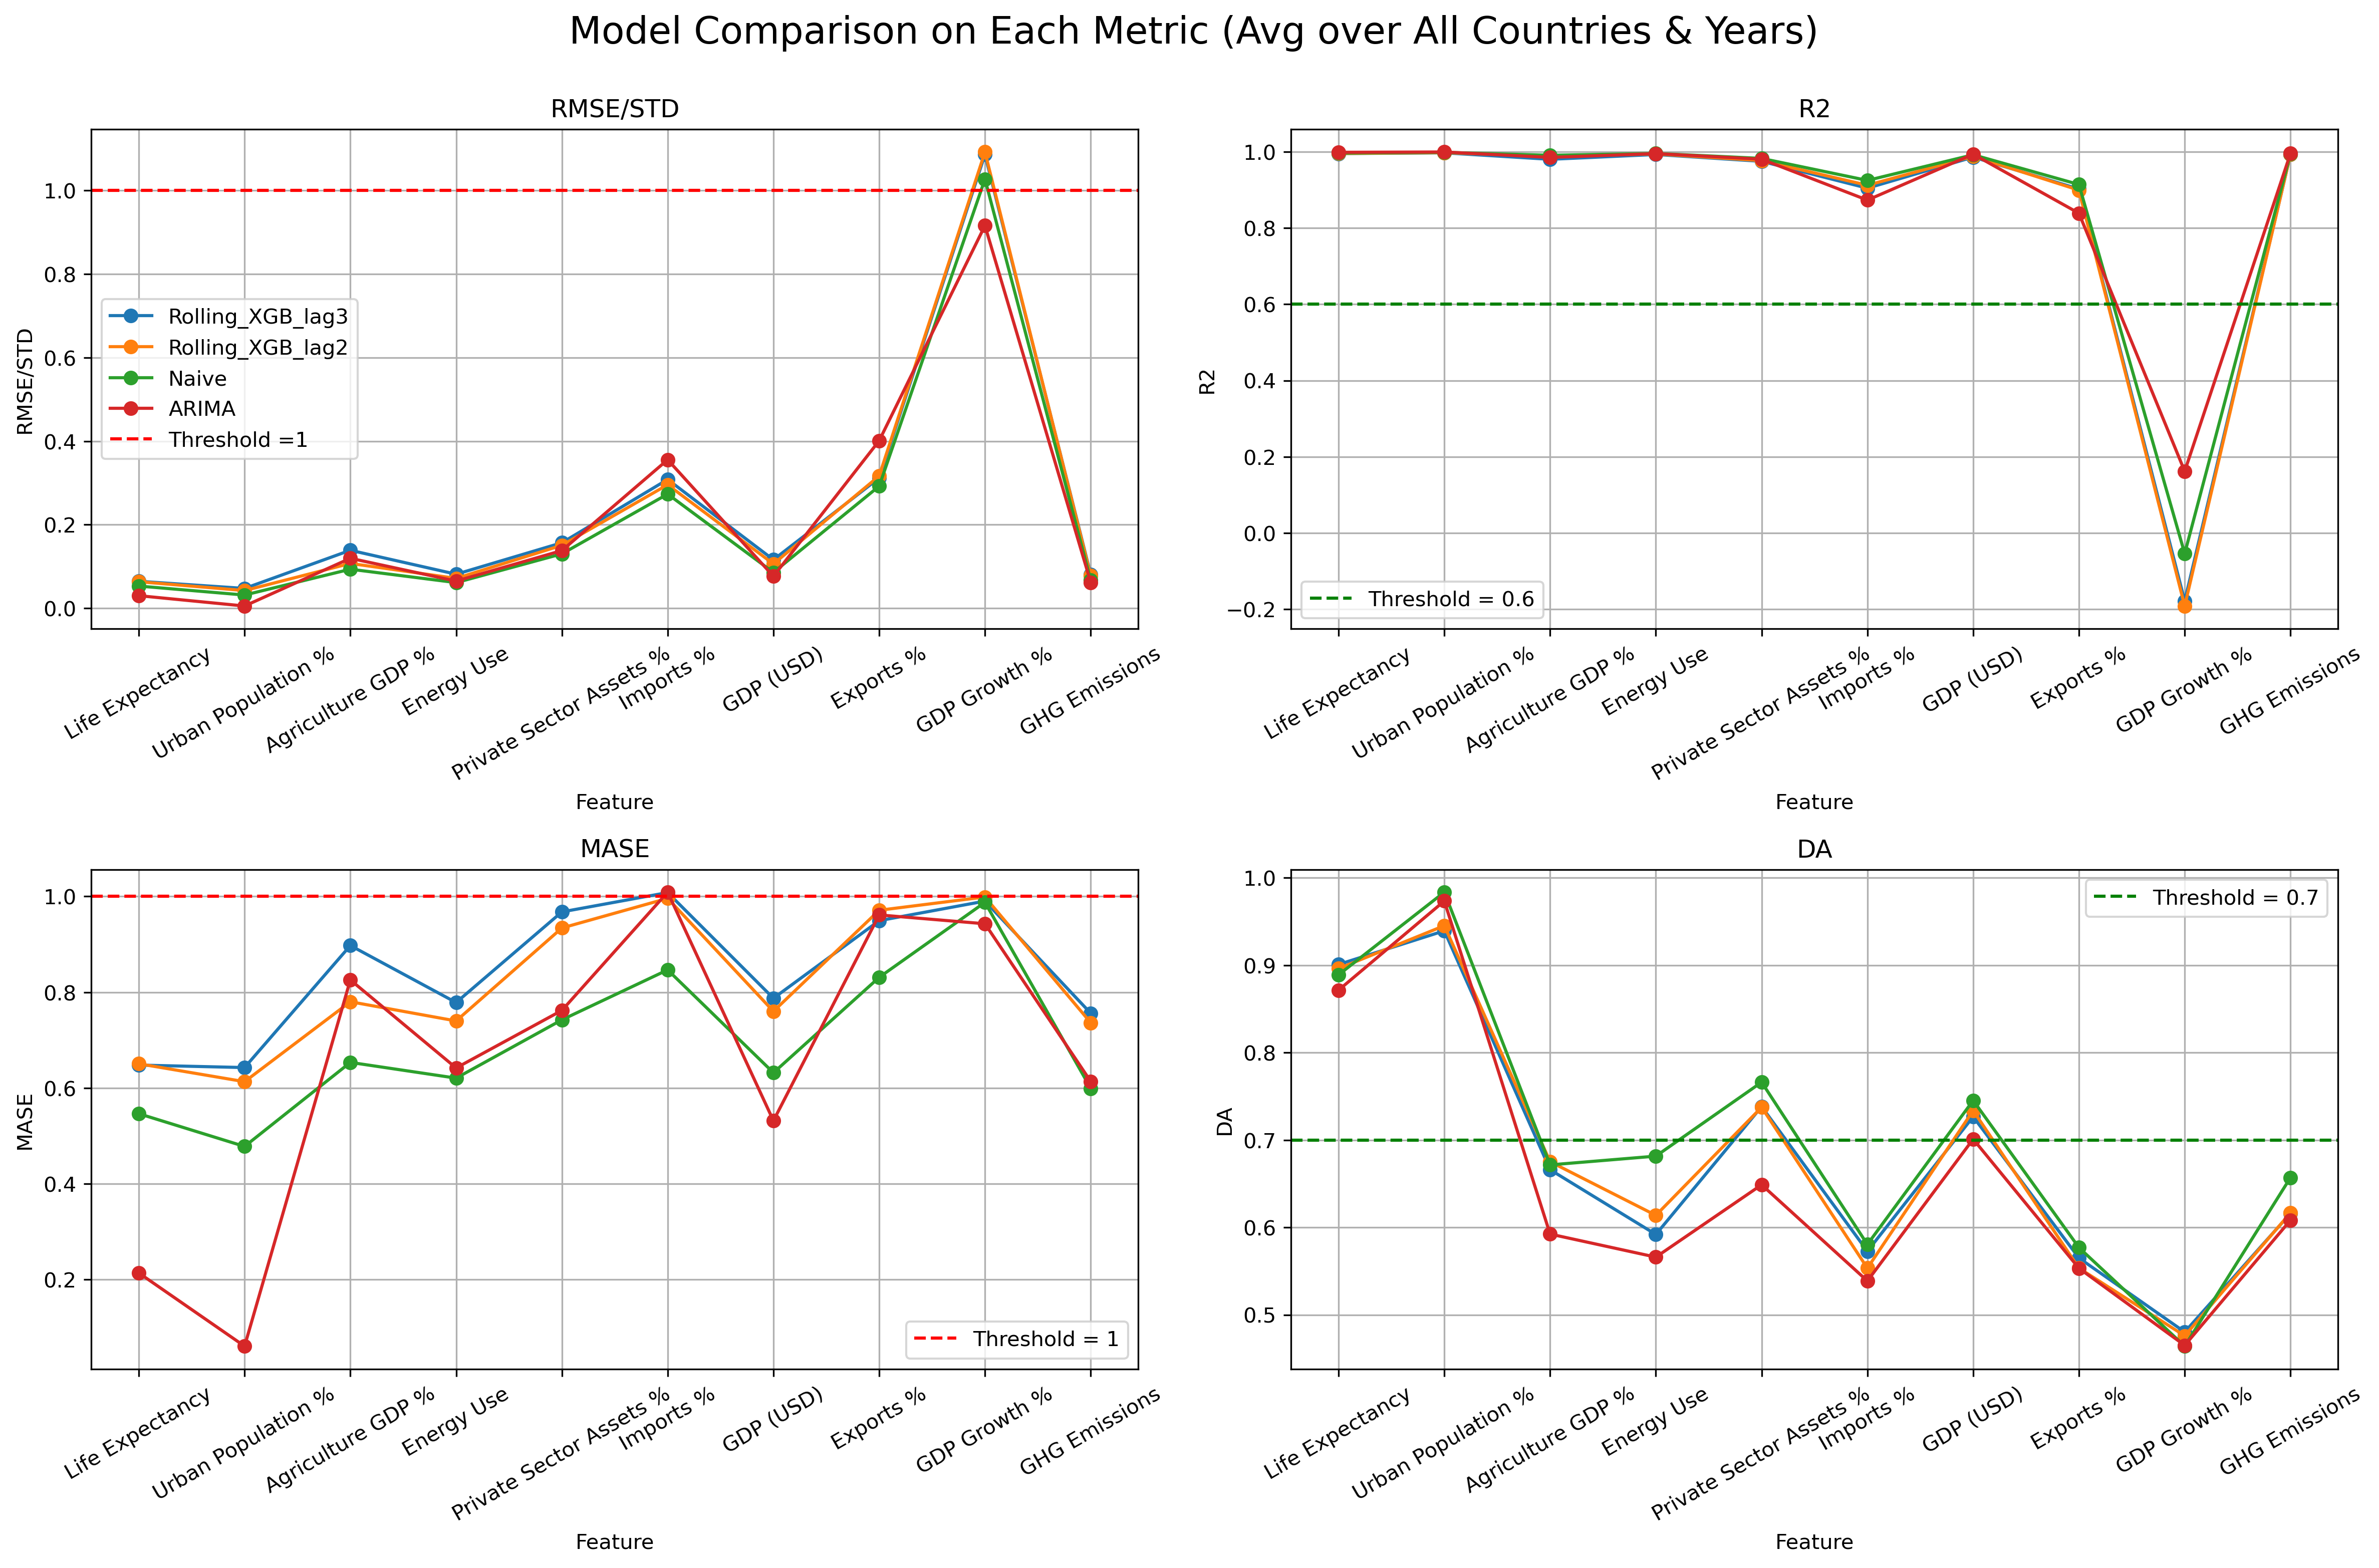
\includegraphics[width=\textwidth]{featurewise_model_comparison.png}
    \caption{Comparison of model performance across indicators using four metrics: RMSE/STD, $R^2$, MASE, and Directional Accuracy (DA). }
    \label{fig:indicator_comparison}
\end{figure}

\begin{figure}[h]
    \centering
    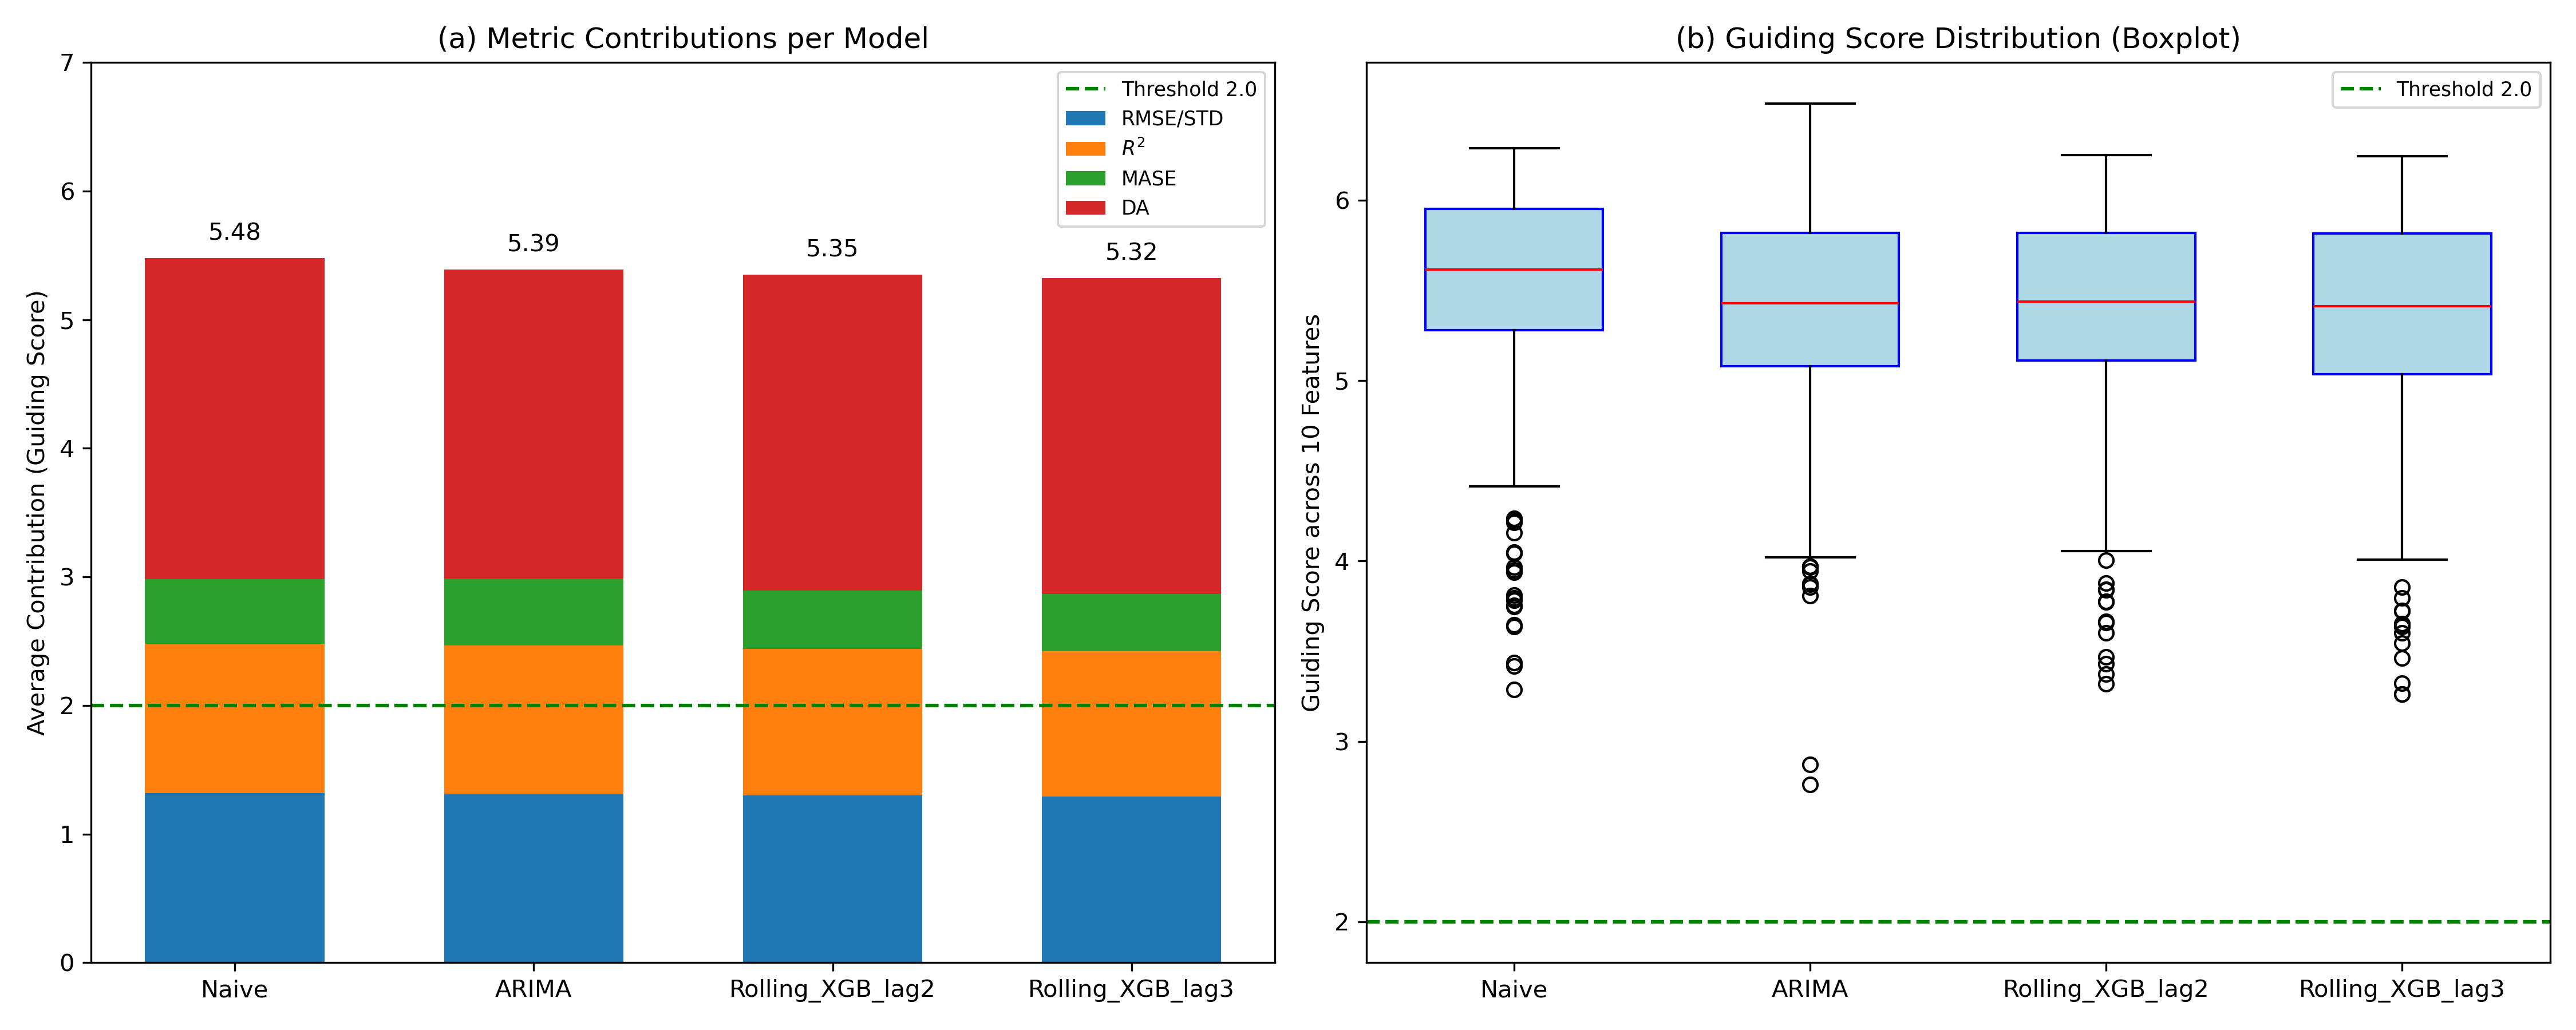
\includegraphics[width=\textwidth]{guiding_score_combined.png}
    \caption{Left figure shows comparison of model performance across indicators using guiding metric. Right figure shows the distribution of guiding scores for each model.}
    \label{fig:indicator_comparison_2}
\end{figure}
We identify three key findings:

First, the Naive Forecast ranks first in Directional Accuracy (DA) for nearly all features, which directly elevates its overall guiding score. This can be attributed to the fact that most national economic indicators—except GDP growth—tend to evolve steadily over short time horizons. In other words, $F_i^{(j)}$ for a feature $i$ in year $j$ is approximately a linear function of $j$, resulting in similar signs between the predicted change $\Delta F_i = F_i^{(j)} - F_i^{(j-1)}$ and the actual change $\Delta F_i' = F_i^{(j+1)} - F_i^{(j)}$. Because our guiding metric assigns the highest weight ($\beta$=5) to DA, the Naive method, despite its simplicity, achieves the top overall score. This inertia-driven advantage is also supported by economic theory. According to structural transformation theory \cite{Kuznets1971}, indicators such as urbanization, agricultural share, and energy use follow stable, long-term trajectories during development, making them easier to predict directionally using simple heuristics.

Second, across the other three metrics—RMSE/STD, $R^2$, and MASE—all four models (Naive, ARIMA, Rolling XGB lag2, and lag3) exhibit comparable performance. As shown in Figure~\ref{fig:indicator_comparison_2} (left), their average scores in these dimensions differ only marginally. Furthermore, Figure~\ref{fig:indicator_comparison} supports this result: most features surpass the threshold for RMSE/STD and $R^2$, indicating strong performance across the board, but fall short in MASE when predicting volatile indicators such as GDP growth. This aligns with prior literature underscoring the unpredictability of economic growth due to policy shifts, external shocks, and cyclical disturbances \cite{Loungani2001}.

Finally, the boxplot in Figure~\ref{fig:indicator_comparison_2} (right) reveals substantial differences in distribution. Although the Naive Forecast has the highest median score and a compact interquartile range, it also produces more low-score outliers. ARIMA yields the highest maximum scores and performs exceptionally well on trend-dominated features like urbanization, benefiting from its built-in trend and seasonality components. However, it also exhibits the widest variance, indicating less robustness. Rolling XGB models show tighter distributions and fewer outliers, suggesting better generalization in high-dimensional, nonlinear contexts. Their advantage lies in modeling complex interactions among indicators—an area where tree-based ML models excel \cite{Athey2019ML, Mullainathan2017ML}.

These findings highlight the critical role of DA in short-term forecasting and suggest that simple methods can remain competitive when variables evolve monotonically. Conversely, complex models offer better scalability for non-stationary or feature-rich environments. Future improvements may include volatility-aware or Bayesian structural break models \cite{stock2002structural, Koop2013Bayesian} to better capture unpredictable features like GDP growth.


% ------------------------------ Figure 7 Analysis ------------------------------
\subsubsection*{Indicator-Specific Feasibility by Country}


\begin{figure}[H]
    \centering
    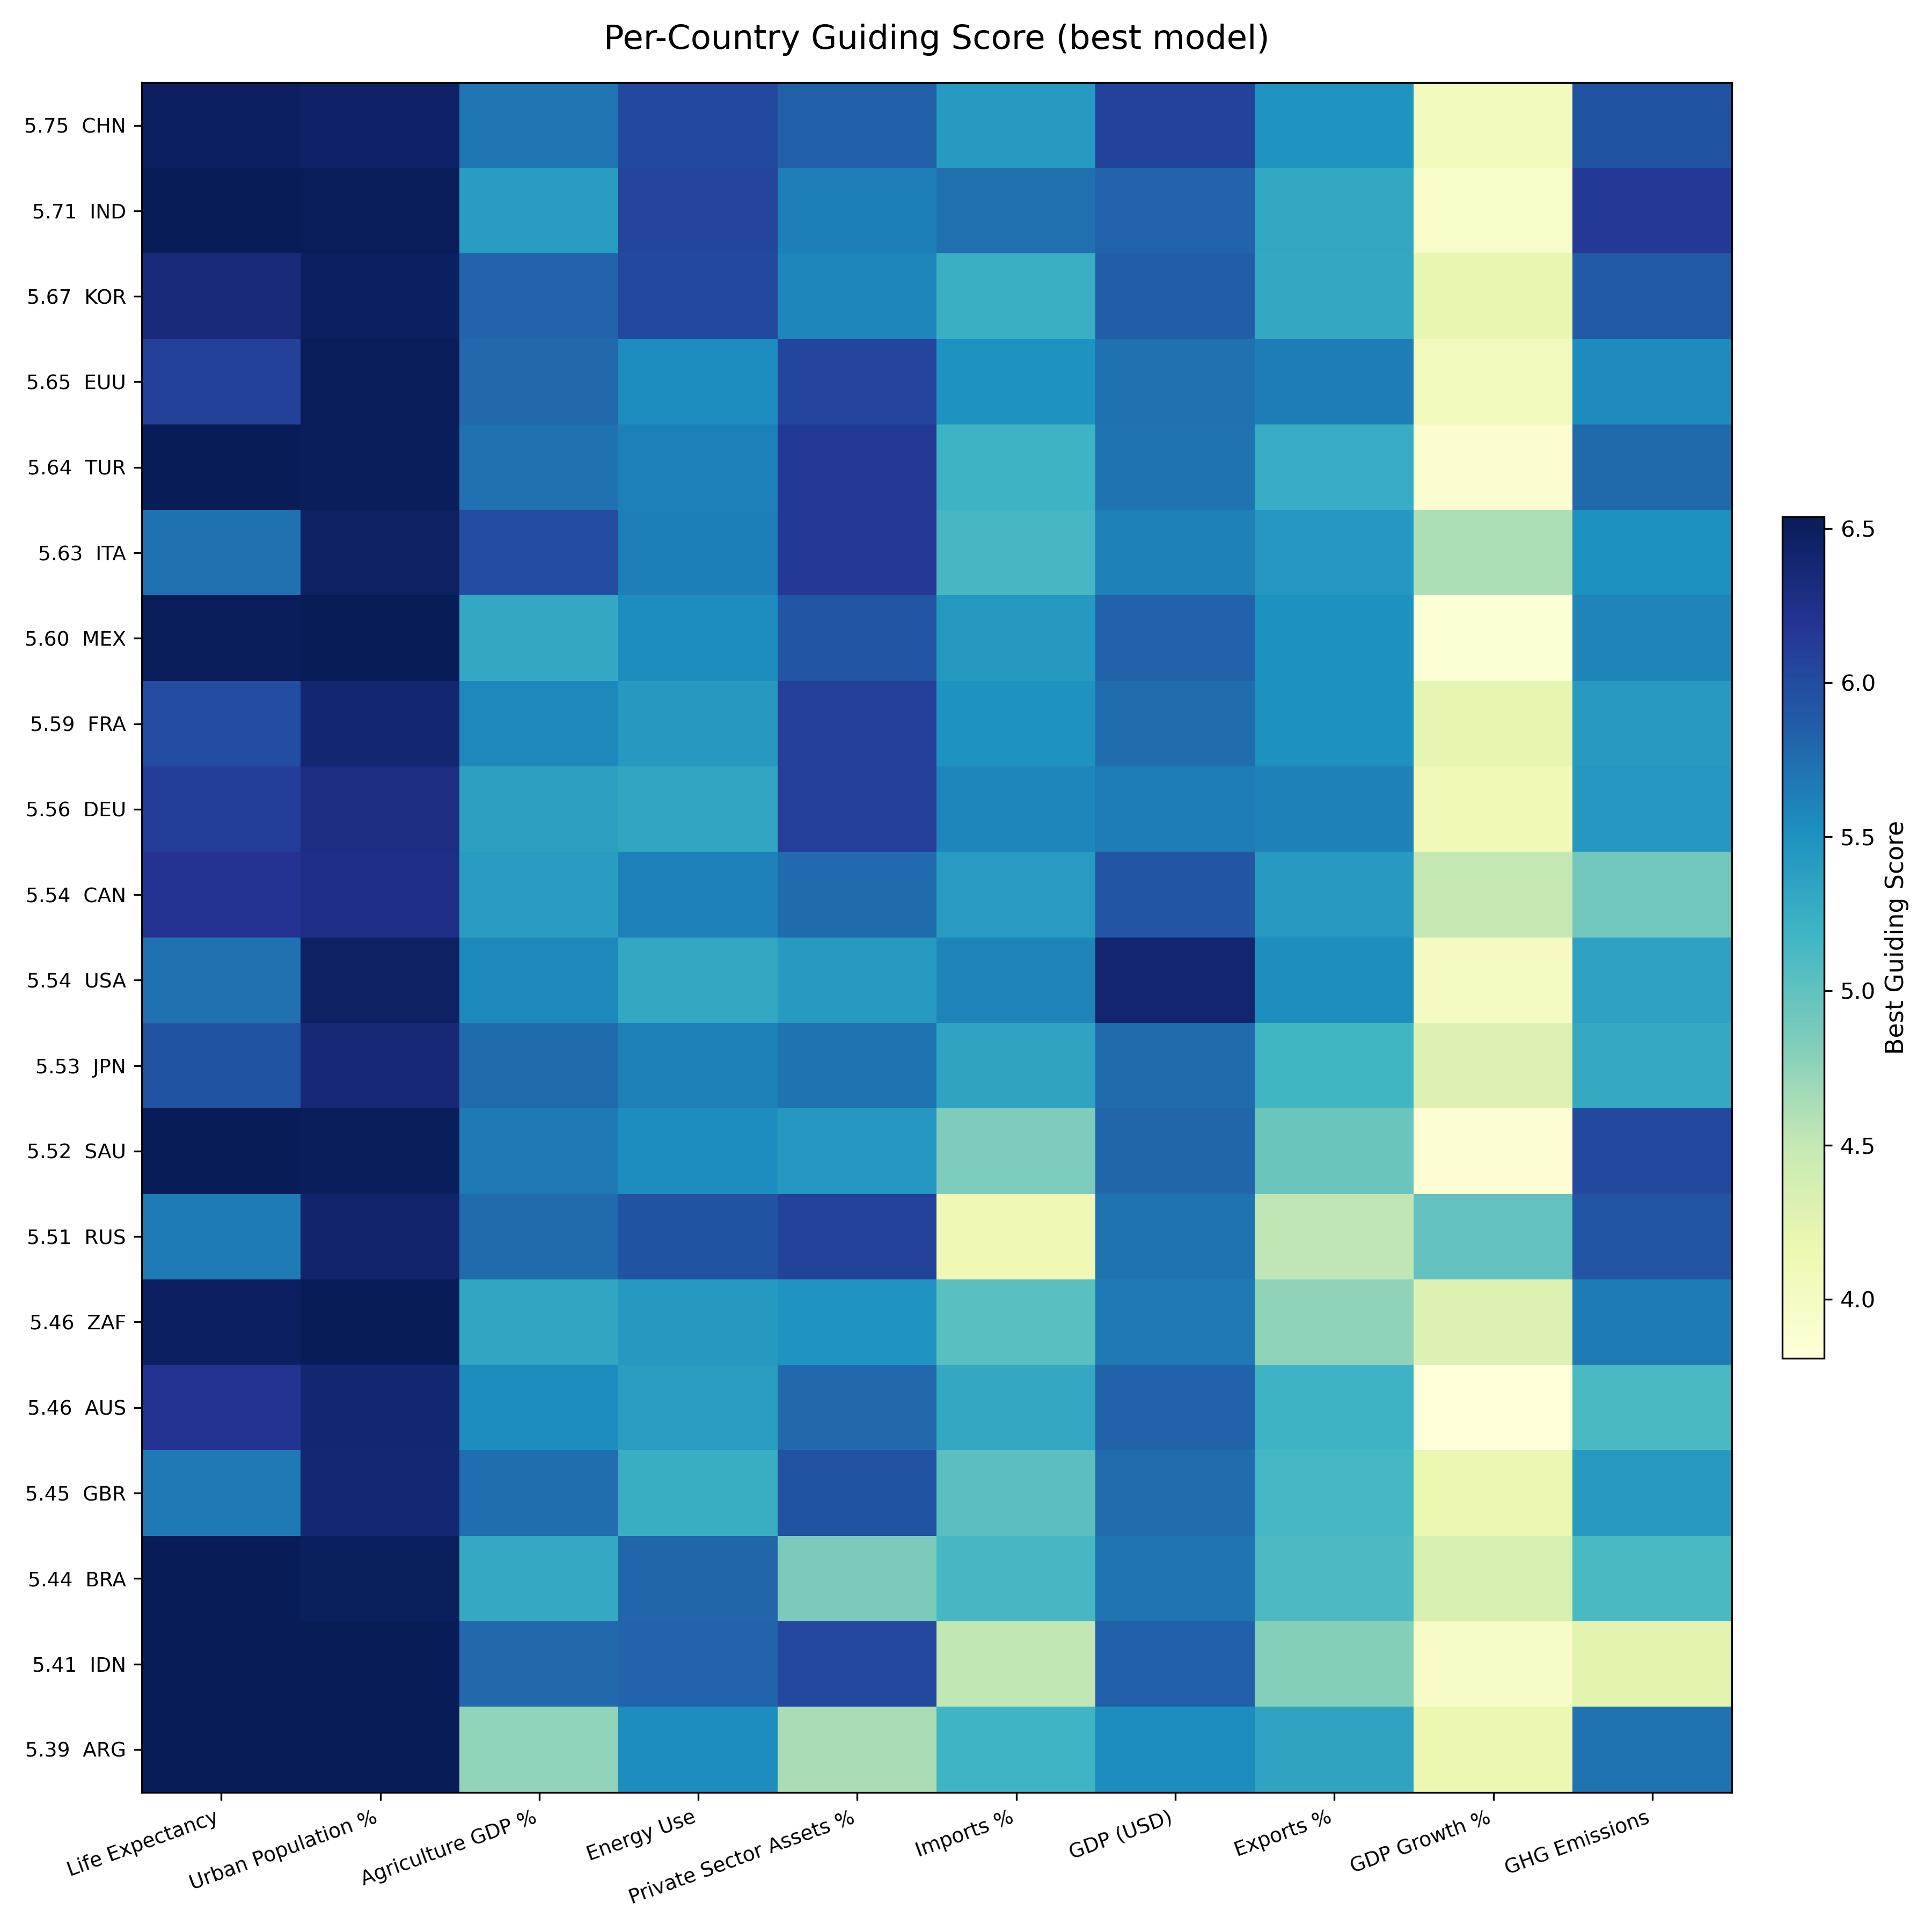
\includegraphics[width=\textwidth]{heat_map.png}
    \caption{Heatmap of Per-Indicator Feasibility Scores by Country. For each (country, indicator) pair, we select the best-performing model and report the corresponding guiding score. Darker colors indicate more reliable prediction.}
    \label{fig:heatmap_feasibility}
\end{figure}


Figure~\ref{fig:heatmap_feasibility} provides a granular view of how forecastability varies both across indicators and across economies.

Three patterns stand out. 

\textbf{(i) Structural indicators are universally easy to predict.} Life expectancy and urban‑population share (first two columns) display uniformly dark shades across nearly every country, reflecting their smooth, monotonic trajectories and the ability of even simple models to capture them. This observation is consistent with the “conditional convergence” hypothesis for demographic and infrastructure variables \cite{Barro1992Convergence}.

\textbf{(ii) Macro‑financial variables exhibit strong cross‑country heterogeneity.} Columns for private‑sector assets, exports, and imports appear markedly lighter for commodity‑oriented economies such as RUS \cite{Prebisch1950, SachsWarner2001} and IDN \cite{VanDerPloegPoelhekke2009} —an outcome that mirrors the high terms‑of‑trade volatility typical of resource‑dependent growth \cite{Prebisch1950}. 
In contrast, advanced economies with diversified trade baskets—such as Germany (DEU), Japan (JPN), and the United States (USA)—achieve guiding scores above 5.5, consistent with IMF Article IV evidence that their external sectors are broadly diversified and less sensitive to commodity-price swings \cite{IMF2023Germany, IMF2023Japan, IMF2023USA}.
However, note that countries with the highest guiding scores generally submit more complete data series to the World Bank; the reduced need for interpolation in turn lowers measurement error and boosts forecast reliability.

\textbf{(iii) GDP growth remains the Achilles’ heel of economic forecasting.} The penultimate column is the lightest for almost every country, reaffirming our earlier conclusion that growth is intrinsically noisy and difficult to pin down. Even for historically steady performers such as CHN or IND, the best guiding score rarely exceeds 4.2. This pattern echoes the well‑documented “growth‑forecast puzzle” discussed by \cite{Loungani2001}.

Taken together, Figure~\ref{fig:heatmap_feasibility} suggests 
that cross‑country heterogeneity in forecastability is driven
 less by modelling technique and more by structural economic 
 characteristics—specifically, the degree of exposure to external 
 shocks and the maturity of demographic transitions. Policymakers 
 can thus place greater confidence in forecasts for slow‑moving 
 structural variables, while treating projections for volatile 
 indicators with appropriate caution.

\subsection{Case Study: G7 and EU}
\begin{figure}[H]
    \centering
    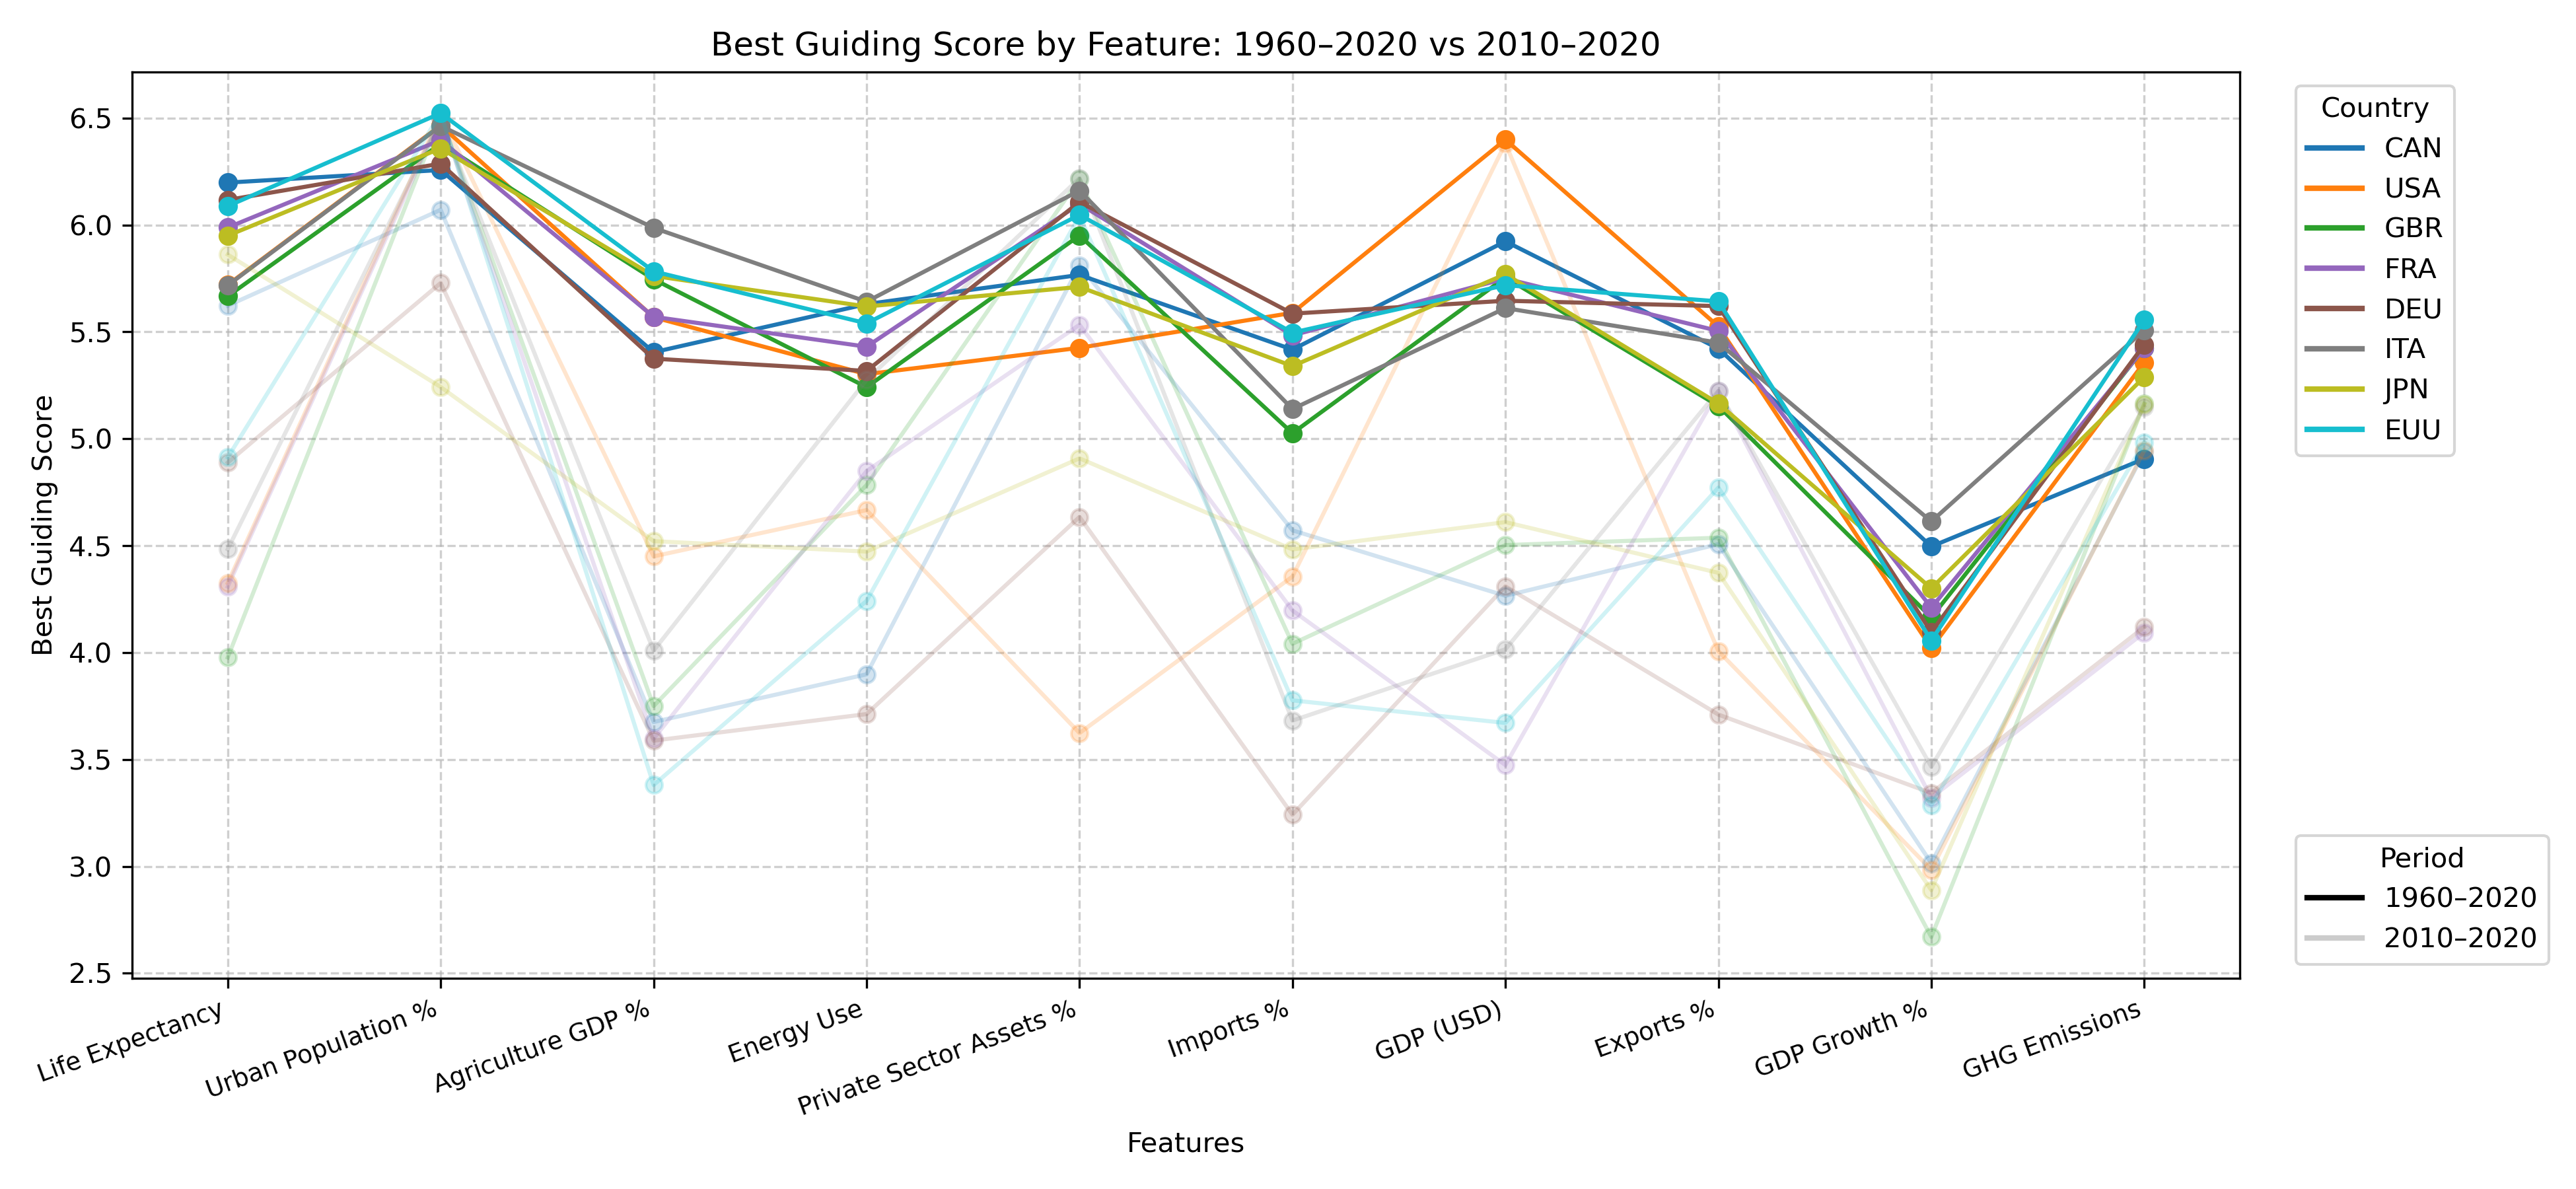
\includegraphics[width=\textwidth]{comparison_feature_G7&EU.png}
\caption{Guiding Score comparison across key indicators for selected G7 and EU countries. Each polyline represents a country, with higher scores indicating more reliable prediction. Solid lines correspond to the full period (1960–2020), while faded lines represent the recent decade (2010–2020).}    
\label{fig:CaseStudyG7EU}
\end{figure}

Figure~\ref{fig:CaseStudyG7EU} reinforces earlier findings: life expectancy and 
urban population share remain the most predictable indicators, 
with scores exceeding 5.5 and 6.0 across all countries and time periods. 
In contrast, GDP growth consistently exhibits the lowest scores, 
rarely surpassing 4.5, confirming its volatility~\cite{Loungani2001}. 
Most G7 economies show minimal performance drop between the two time periods, 
indicating data stability and model robustness over time. 

\subsection{Case Study: BRICS-5}
\begin{figure}[h]
    \centering
    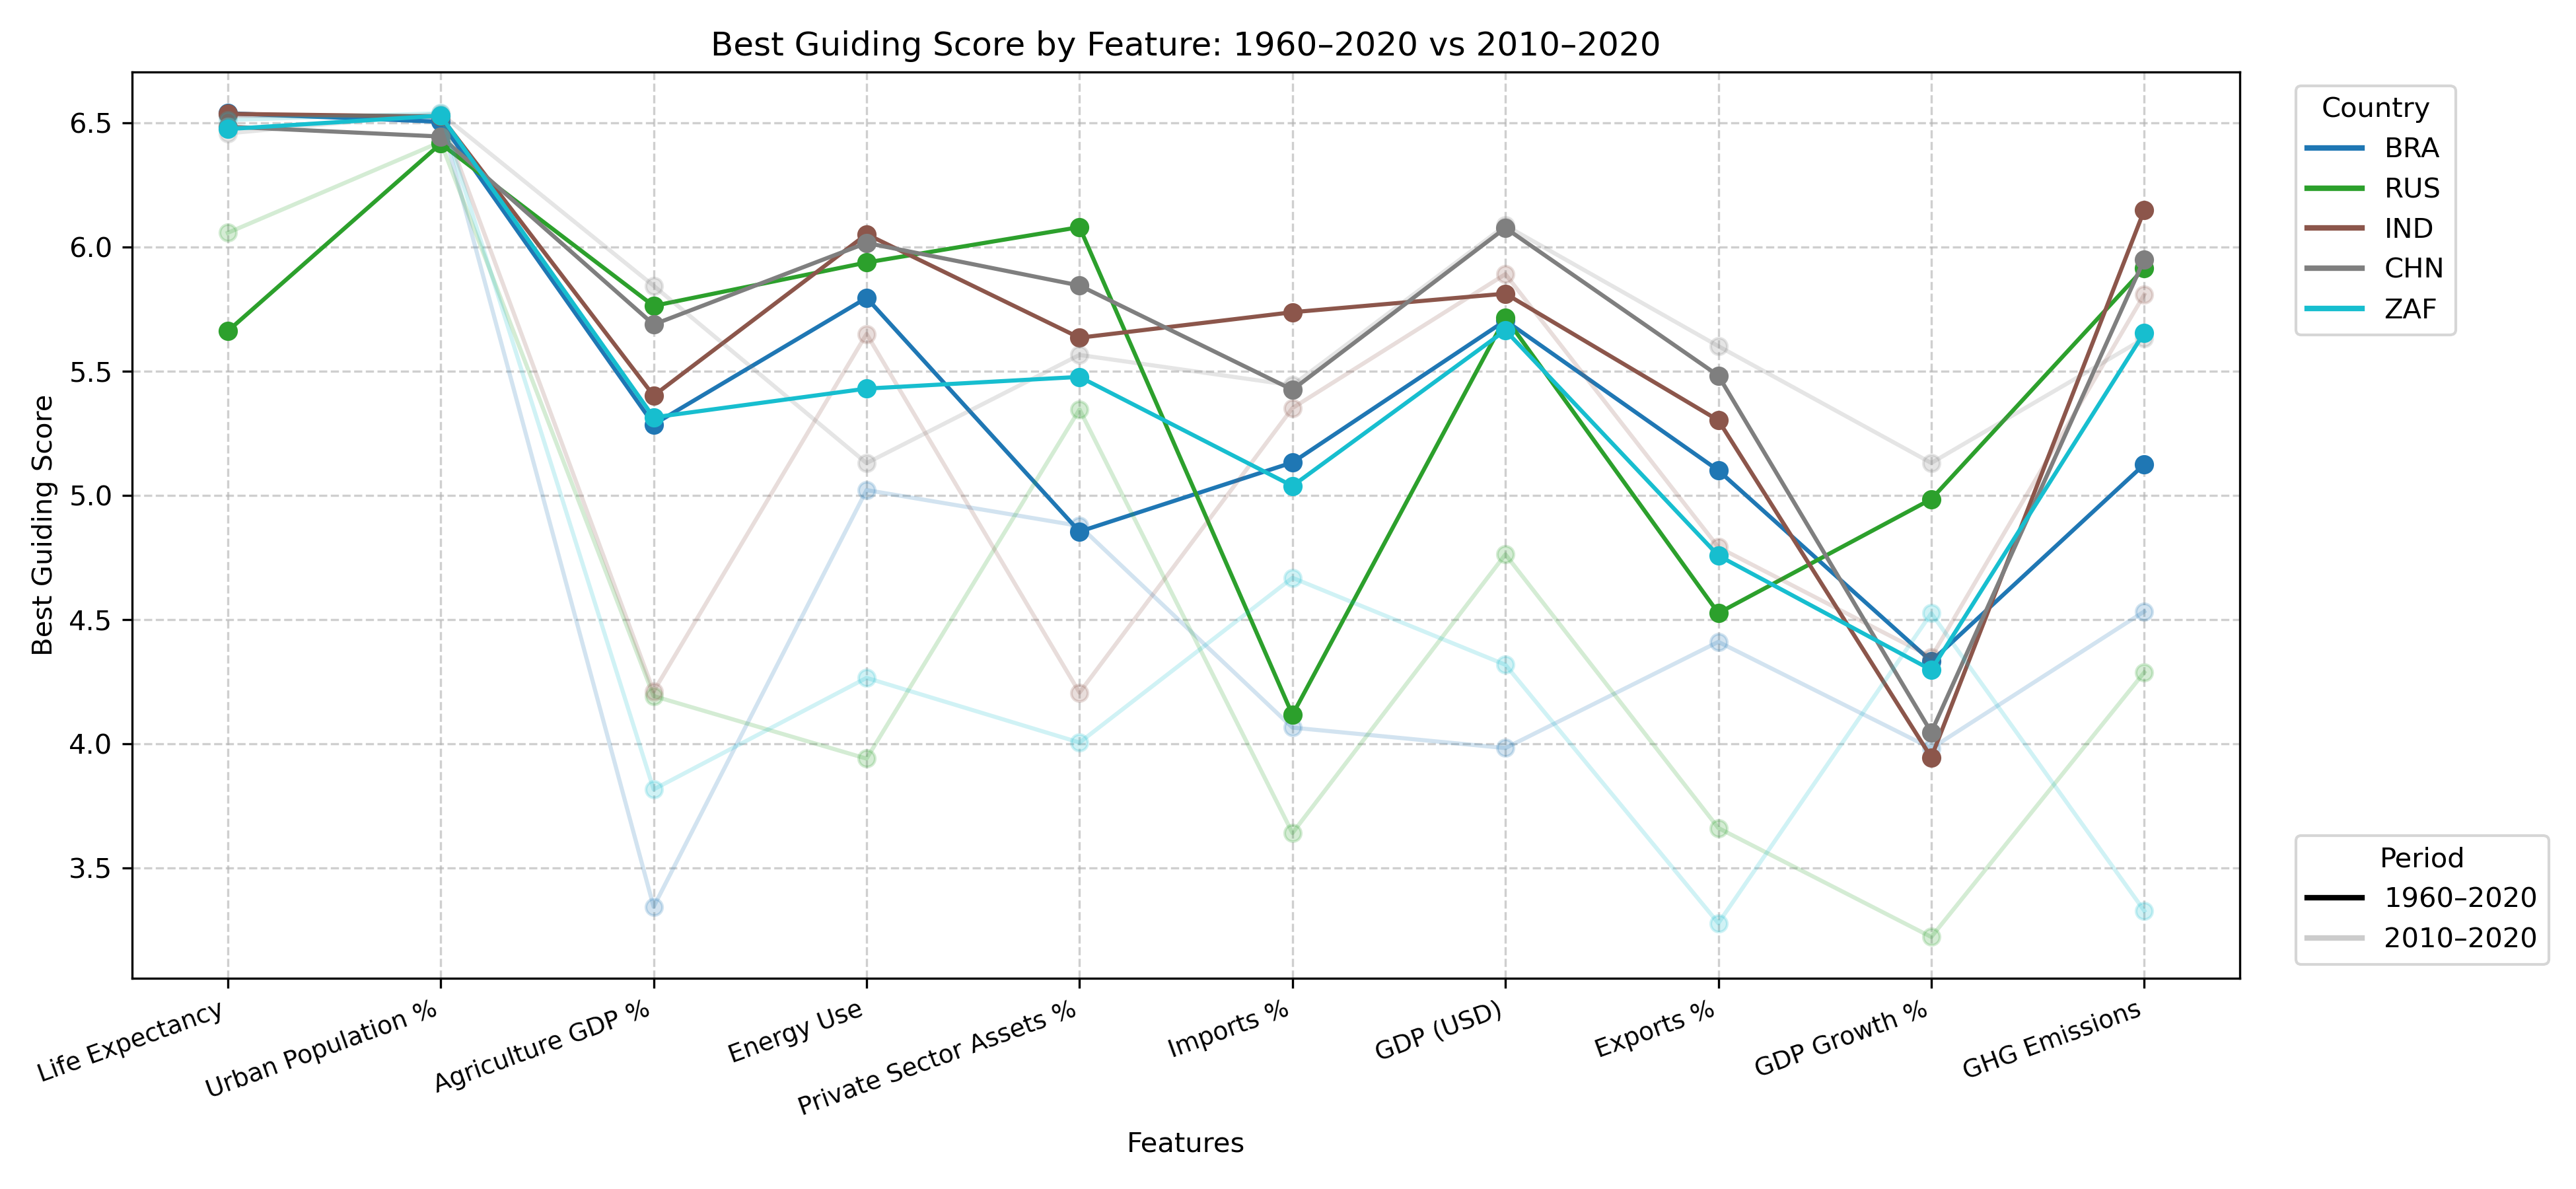
\includegraphics[width=\textwidth]{comparison_feature_BRICS.png}
\caption{Guiding Score comparison across key indicators for BRICS-5 countries (Brazil, Russia, India, China, South Africa). }    
\label{fig:CaseStudyBRICS5}
\end{figure}
From Figure~\ref{fig:CaseStudyBRICS5}, structural indicators again 
 stand out: urbanization and life expectancy exceed the guiding threshold 
 of 5.5 and 6.0 across all five countries. However, BRICS economies display greater 
 cross-feature and cross-period variation, especially for financial 
 indicators like private sector assets and exports, reflecting their more 
 dynamic and transitional economic structures~\cite{Lin2012newstructural}. 
 India and South Africa exhibit sharper declines in the recent decade (2010–2020), 
 likely due to external shocks and data limitations. 
 The persistently low scores for GDP growth echo global 
 patterns and further underscore the limits of model-based forecasting 
 for cyclical variables~\cite{ClementsHendry2002}.



% --- Begin Chapter 6 ---
% --- Begin Chapter 6 ---
% --- Begin Chapter 6 ---
\section{Bayesian Latent Structure Model for Multi-Country Economic Forecasting}

\subsection{Model Motivation and Setup}

\paragraph{Notation and Dimensions.}
Let $m$ be the number of features and $n$ the number of countries. For each country $c$ at time $t$, let $\mathbf{Y}_{t,c} \in \mathbb{R}^m$ be the observed feature vector. Define a fixed feature mask $\mathcal{I} \subseteq \{1, \ldots, m\}$ of size $d$ (e.g., import/export-related indices) used for cross-country influence. For any country $j$, define $\mathbf{Z}_{t,j} \in \mathbb{R}^m$ by setting:
\[
\left(\mathbf{Z}_{t,j}\right)_i = 
\begin{cases}
\left(\mathbf{Y}_{t,j}\right)_i & \text{if } i \in \mathcal{I} \\
0 & \text{otherwise}
\end{cases}
\]
For any country $c$, define the stacked cross-feature matrix $X_{t,c} \in \mathbb{R}^{(n-1) \times m}$ as:
\[
X_{t,c} = \begin{bmatrix}
\mathbf{Z}_{t-1,1}^\top \\
\vdots \\
\mathbf{Z}_{t-1,c-1}^\top \\
\mathbf{Z}_{t-1,c+1}^\top \\
\vdots \\
\mathbf{Z}_{t-1,n}^\top
\end{bmatrix}
\]

In this chapter, we propose a Bayesian latent structure framework designed to forecast key economic indicators across multiple countries by integrating time-lagged dependencies and cross-national interactions. Our approach aims to strike a balance between interpretability, forecasting accuracy, and theoretical grounding.

Let $\mathbf{Y}_{t,c}$ denote the standardized vector of economic indicators for country $c$ in year $t$. We assume the observed data can be explained by latent shared influences through a generative model of the form:
\[
\mathbf{Y}_{t,c} = \sum_{i=1}^\tau  A_{t,c}^i \mathbf{Y}_{t - i,c} + \sum_{j \neq c} M_{j,c} \mathbf{Z}_{t-1,j} + \boldsymbol{\epsilon}_{t,c}, \quad \boldsymbol{\epsilon}_{t,c} \sim \mathcal{N}(\mathbf{0}, \sigma^2 I)
\]

Here, the dimensions of the variables are as follows: 
$\mathbf{Y}_{t,c} \in \mathbb{R}^m$ represents the observed indicators for country $c$ at time $t$, 
$A_{t,c} \in \mathbb{R}^{m \times m}$ is the transition matrix for self-history, 
$M_{j,c} \in \mathbb{R}^{m \times m}$ maps the external features $\mathbf{Z}_{t-1,j} \in \mathbb{R}^m$ from country $j$ to the output space, 
and $\boldsymbol{\epsilon}_{t,c} \in \mathbb{R}^m$ is the noise term.

The model incorporates three main components:
\begin{itemize}
  \item \textbf{Self-History Influence:} We include the past $\tau$ years of the country's own indicators $\mathbf{Y}_{t-i,c}$, aggregated with exponentially weighted powers of matrix $A$. To ensure diminishing influence over time and model stability, we assume $\det A < 1$.
  \item \textbf{Cross-Country Influence:} For external effects, we use the sparse cross-feature vectors $\mathbf{Z}_{t-1,j} \in \mathbb{R}^m$ as defined above, with only a predefined subset of $d$ components (corresponding to selected cross features) nonzero. This sparse representation ensures that $\mathbf{Z}$ has the same dimension as $\mathbf{Y}$, but only encodes relevant cross-national influences. We define a set of matrices $\{M_{j,c} \in \mathbb{R}^{m \times m} \mid j \neq c\}$ that model how the retained features from each country $j$ influence the target country $c$. The total cross-country effect is computed as:
  \[
  \sum_{j \neq c} M_{j,c} \mathbf{Z}_{t-1,j}
  \]
  This setup allows each $M_{j,c}$ to focus on relevant dimensions, while preserving compatibility with $\mathbf{Y}_{t,c}$.
  \item \textbf{Noise Term:} The additive noise $\boldsymbol{\epsilon}_{t,c}$ accounts for unexplained variability, assumed to be i.i.d. Gaussian with zero mean and isotropic covariance.
\end{itemize}

In this paper, we select $\tau = 2$ based on empirical evidence that XGB\_lag2 and XGB\_lag3 models show minimal performance difference in earlier experiments, indicating that higher powers of $A$ (i.e., $A^3$ and beyond) have negligible contribution. We set $d = 2$ to focus on two key cross-country indicators—import and export proportions—which capture essential aspects of international economic interactions.


In this formulation, we assume a uniform cross-country influence mechanism across all countries, which allows simplification in later estimation steps.


% --- Section 6.2: Model Estimation and Inference ---
\subsection{Simplified Estimation with Shared Cross-Country Influence}

\subsubsection*{6.2.1 Assumptions and Notation}

We assume that all countries share the same cross-country influence weights $M \in \mathbb{R}^{m \times m}$ applied to a masked cross-feature sum. This allows us to define:
\[
\mathbf{Q}_{t,c} = \sum_{j \ne c} \mathbf{Z}_{t-1,j}
\]
where each $\mathbf{Z}_{t-1,j}$ is a masked version of $\mathbf{Y}_{t-1,j}$ retaining only $d$ predefined features. The vector $\mathbf{Q}_{t,c} \in \mathbb{R}^m$ is used to represent the aggregated cross-country input for predicting $\mathbf{Y}_{t,c}$.

% 6.2.2 Ridge Regression Estimation (Restored with full mathematical derivation)

 \subsubsection*{6.2.2 Ridge Regression Estimation}

The prediction for each country $c$ at time $t$ is:
\[
\hat{\mathbf{Y}}_{t,c} = A^1 \mathbf{Y}_{t-1,c} + A^2 \mathbf{Y}_{t-2,c} + \sum_{j \ne c} M_j \mathbf{Z}_{t-1,j}
\]
We denote the prediction residual as:
\[
\mathbf{r}_{t,c} = \mathbf{Y}_{t,c} - \hat{\mathbf{Y}}_{t,c}
\]
The objective is to minimize the total loss over all years and countries using a ridge penalty:
\[
\mathcal{L} = \sum_{t,c} \left\| \mathbf{r}_{t,c} \right\|_2^2 + \lambda_A \left( \|A^1\|_F^2 + \|A^2\|_F^2 \right) + \lambda_M \sum_j \|M_j\|_F^2
\]
where $\lambda_A$ and $\lambda_M$ are regularization parameters.

To estimate the parameters, we organize the inputs into a linear model.

For each $(t, c)$, define the concatenated input vector:
\[
\mathbf{h}_{t,c} = \begin{bmatrix}
\mathbf{Y}_{t-1,c}^T \\
\mathbf{Y}_{t-2,c}^T \\
\{\mathbf{Z}_{t-1,j}\}_{j \ne c}^T
\end{bmatrix}
\in \mathbb{R}^{m(\tau + n - 1)}
\]
and corresponding parameter block:
\[
\mathbf{W}_c = \begin{bmatrix}
(A^1)^T \\
(A^2)^T \\
\{M_j\}_{j \ne c}^T
\end{bmatrix}
\in \mathbb{R}^{m(\tau + n - 1) \times m}
\]
The prediction becomes:
\[
\hat{\mathbf{Y}}_{t,c} = \mathbf{W}_c^\top \mathbf{h}_{t,c}
\]
Letting $\mathbf{H}_c$ be the stacked input matrix and $\mathbf{Y}_c$ the corresponding outputs over time:
\[
\mathbf{H}_c = \begin{bmatrix}
\mathbf{h}_{\tau+1, c}^\top \\
\vdots \\
\mathbf{h}_{T, c}^\top
\end{bmatrix}
\in \mathbb{R}^{(T - \tau) \times m(\tau + n - 1)}, \quad
\mathbf{Y}_c = \begin{bmatrix}
\mathbf{Y}_{\tau+1, c}^\top \\
\vdots \\
\mathbf{Y}_{T, c}^\top
\end{bmatrix}
\in \mathbb{R}^{(T - \tau) \times m}
\]
Initially, we set the regularization strength for both the self-influence terms \( A \) and cross-influence terms \( M \) to be the same, i.e., \(\lambda_A = \lambda_M\).
Moreover, we let \(\lambda_A = \lambda_M\ = 1.0\).
Then the objective is:
\[
\mathcal{L}_c = \| \mathbf{Y}_c - \mathbf{H}_c \mathbf{W}_c \|_F^2 + \lambda \| \mathbf{W}_c \|_F^2
\]
and the closed-form ridge solution is:
\[
\mathbf{W}_c = (\mathbf{H}_c^\top \mathbf{H}_c + \lambda I)^{-1} \mathbf{H}_c^\top \mathbf{Y}_c
\]

This simplification facilitates direct estimation using standard ridge regression. The guiding scores of this baseline are shown in Figure~\ref{fig:guiding_score_ridge}.

\begin{figure}[H]
  \centering
  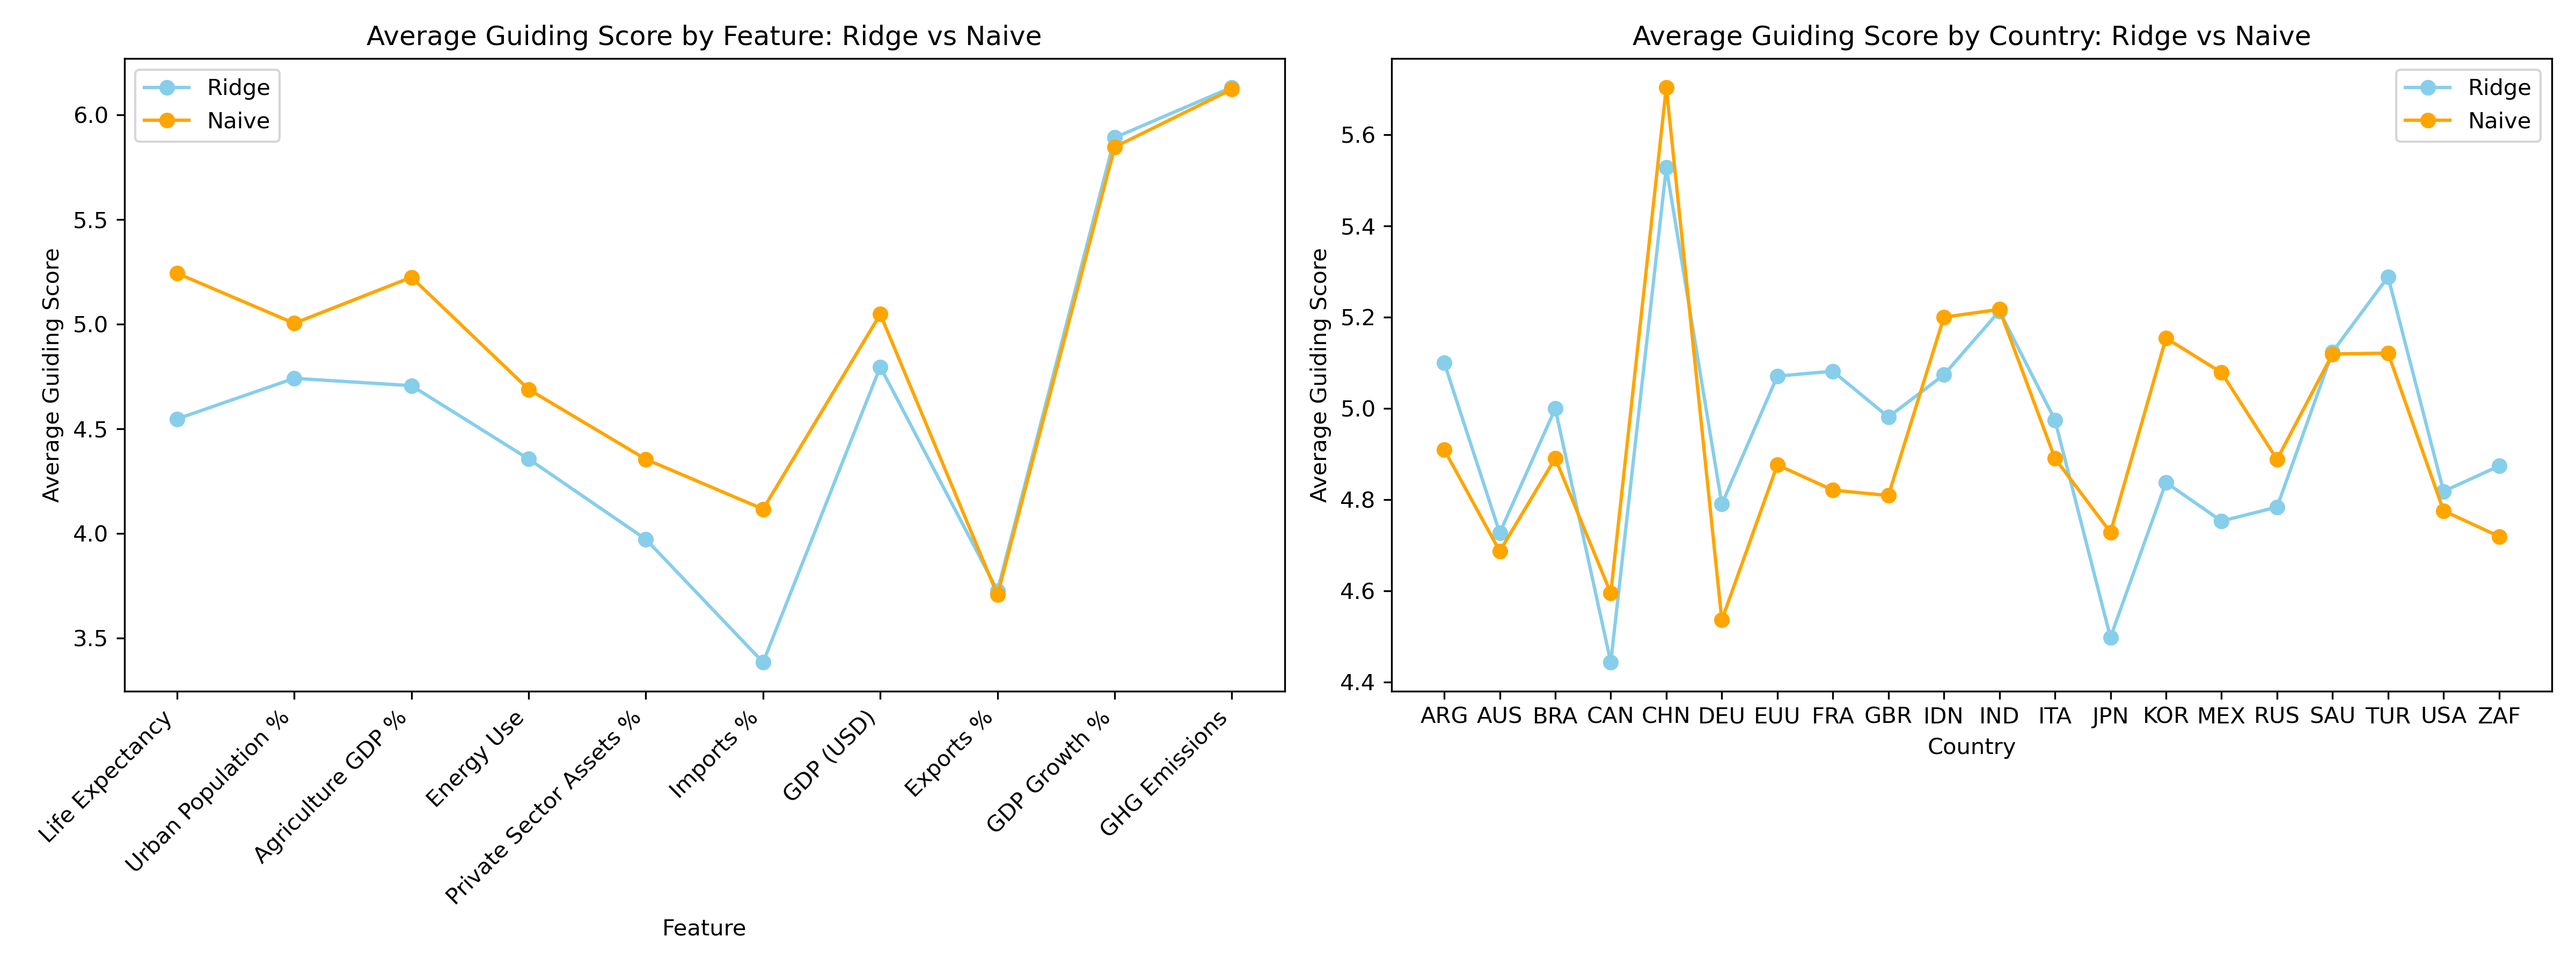
\includegraphics[width=0.9\textwidth]{guiding_score_ridge.png}
  \caption{Guiding scores for Ridge vs Naive using uniform regularization}
  \label{fig:guiding_score_ridge}
\end{figure}

To better capture the different roles of \( A \) and \( M \), we then optimize \(\lambda_A\) and \(\lambda_M\) separately. This allows for more flexible control over self and cross influence regularization strengths. 
The updated guiding score comparison after separate tuning is presented in Figure~\ref{fig:guiding_score_ridge2}.

% --- Inserted: Ridge2 guiding score figure and discussion ---
\begin{figure}[H]
  \centering
  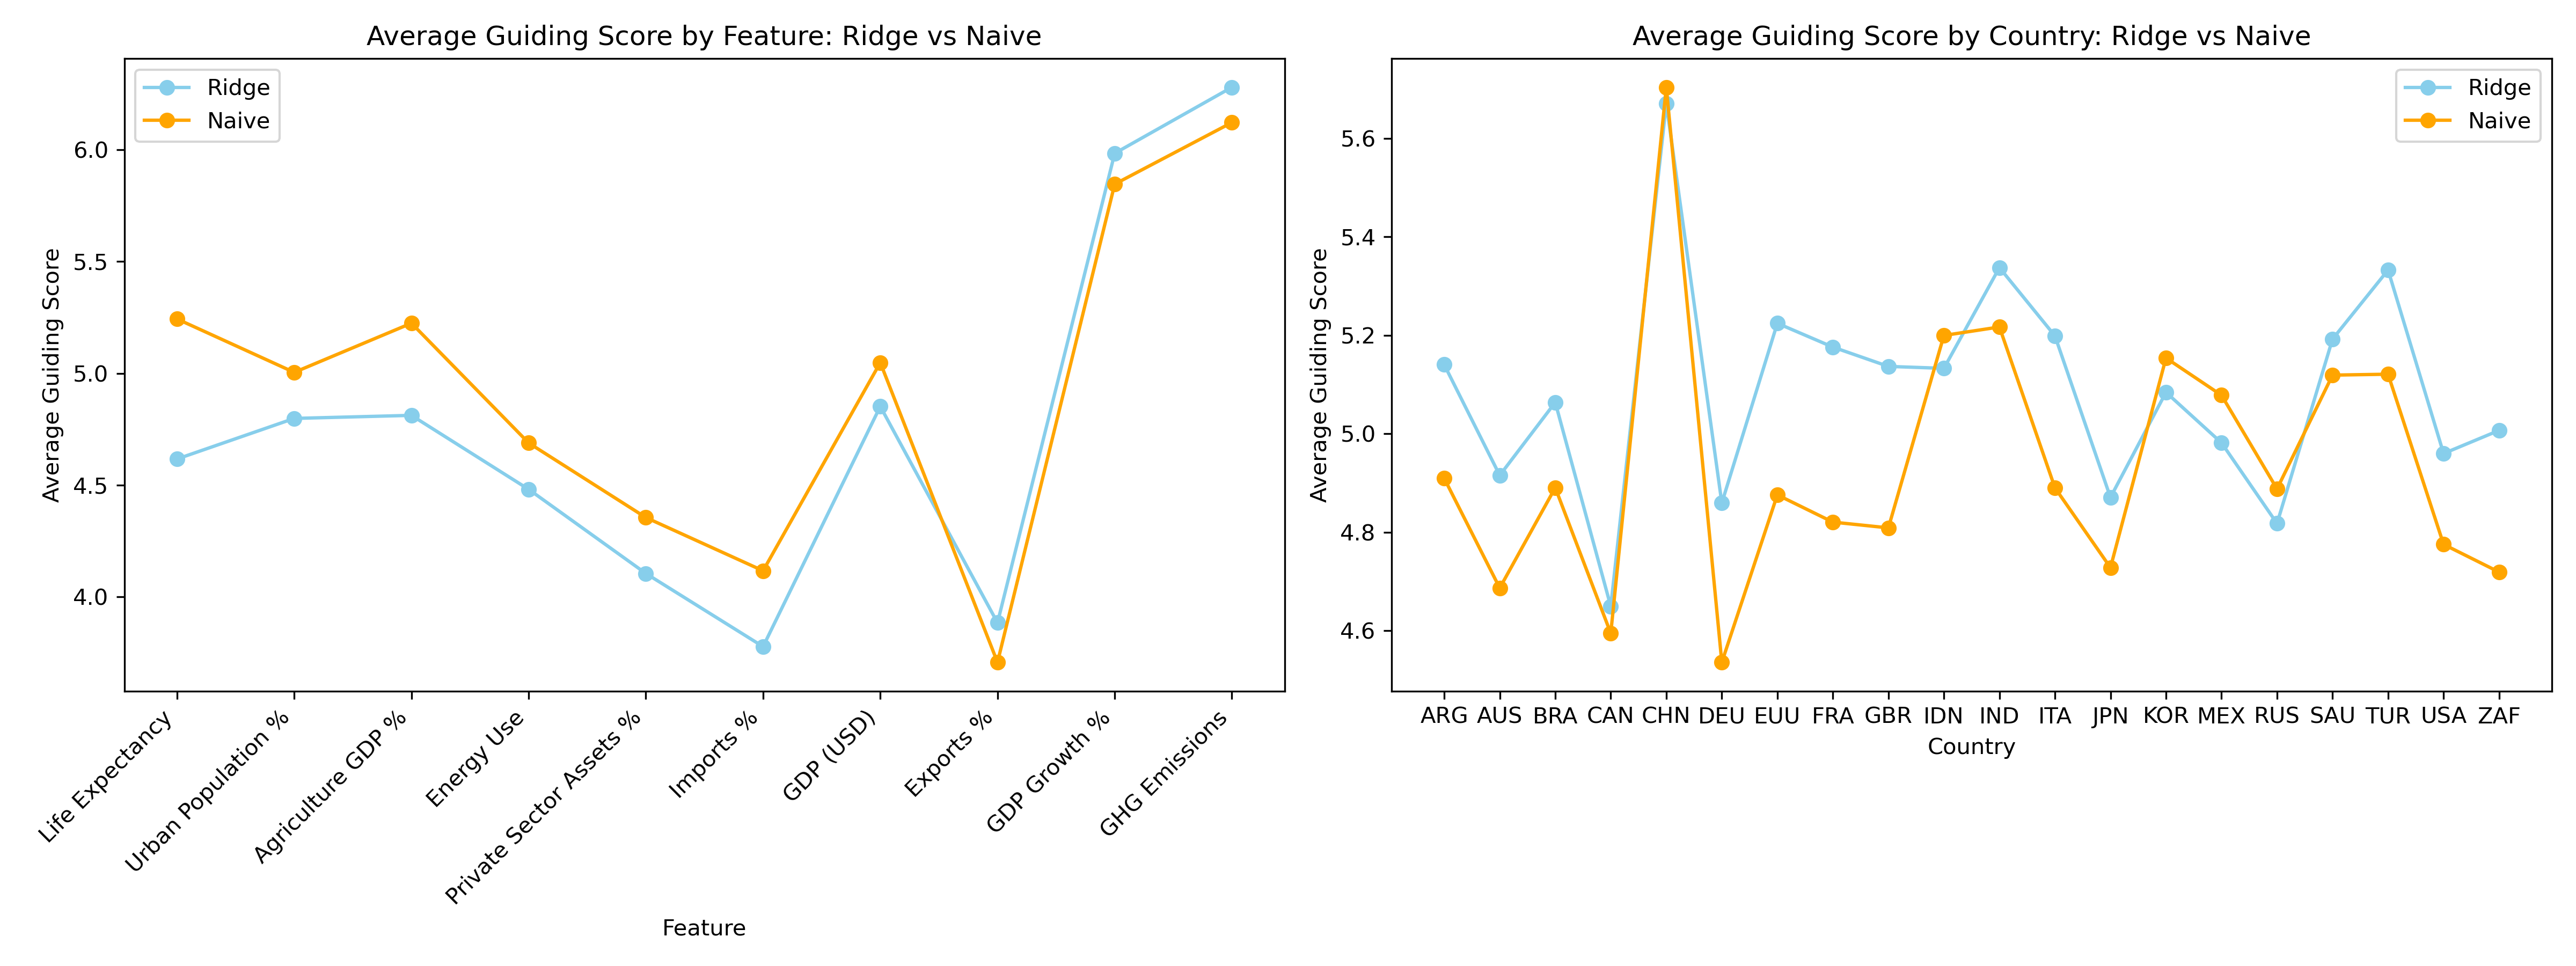
\includegraphics[width=0.9\textwidth]{guiding_score_ridge2.png}
  \caption{Guiding scores after parameter tuning for each (country, feature) pair.}
  \label{fig:guiding_score_ridge2}
\end{figure}

Figure~\ref{fig:guiding_score_ridge2} reveals that tuning $(\lambda_A, \lambda_M)$ for each individual (country, feature) pair yields consistent improvements in guiding score relative to the uniform-regularization baseline in Figure~\ref{fig:guiding_score_ridge}. 
This gain is most apparent for structural indicators and stable countries, where tailored regularization allows the model to better separate temporal inertia from cross-national influences. 

% 6.2.3 Model Evaluation and Visualization (content removed as per instructions)

\subsubsection*{6.2.3 Model Evaluation and Visualization}




% --- Section 6.3: Generalized Cross-Country Modeling ---
\section{Generalized Cross-Country Modeling}

All cross-country influence is encoded by the sum $\mathbf{Q}_{t,c} = \sum_{j \ne c} \mathbf{Z}_{t-1,j}$, preserving structural sparsity while retaining matrix compatibility.

\section{Conclusion}

This work demonstrates that most major structural indicators of national development are highly predictable from a small set of other key indicators, especially when using ensemble tree-based machine learning models. The exception is GDP growth rate, which remains notoriously difficult to forecast—consistent with macroeconomic theory and previous empirical research.

Our results suggest that, for long-run cross-country comparative analysis, reliable prediction of most economic and demographic indicators is feasible using standard machine learning approaches and open-access datasets. However, caution should be exercised when interpreting models for inherently volatile outcomes such as economic growth. Overall, this study highlights the promise and limitations of data-driven prediction in international development research and points to several avenues for further methodological and substantive refinement.


\section*{Project Repository}
The full code, data preprocessing scripts, and results can be found at: [GitHub link will be inserted here].



\bibliographystyle{unsrt}
\bibliography{references}
\end{document}